\sectionframe{Results of my Masters Thesis}
\section{Masters Thesis}

\begin{frame}{Archetypal Model}
	\only<1>{
		\begin{figure}
			\stackunder[5pt]{
				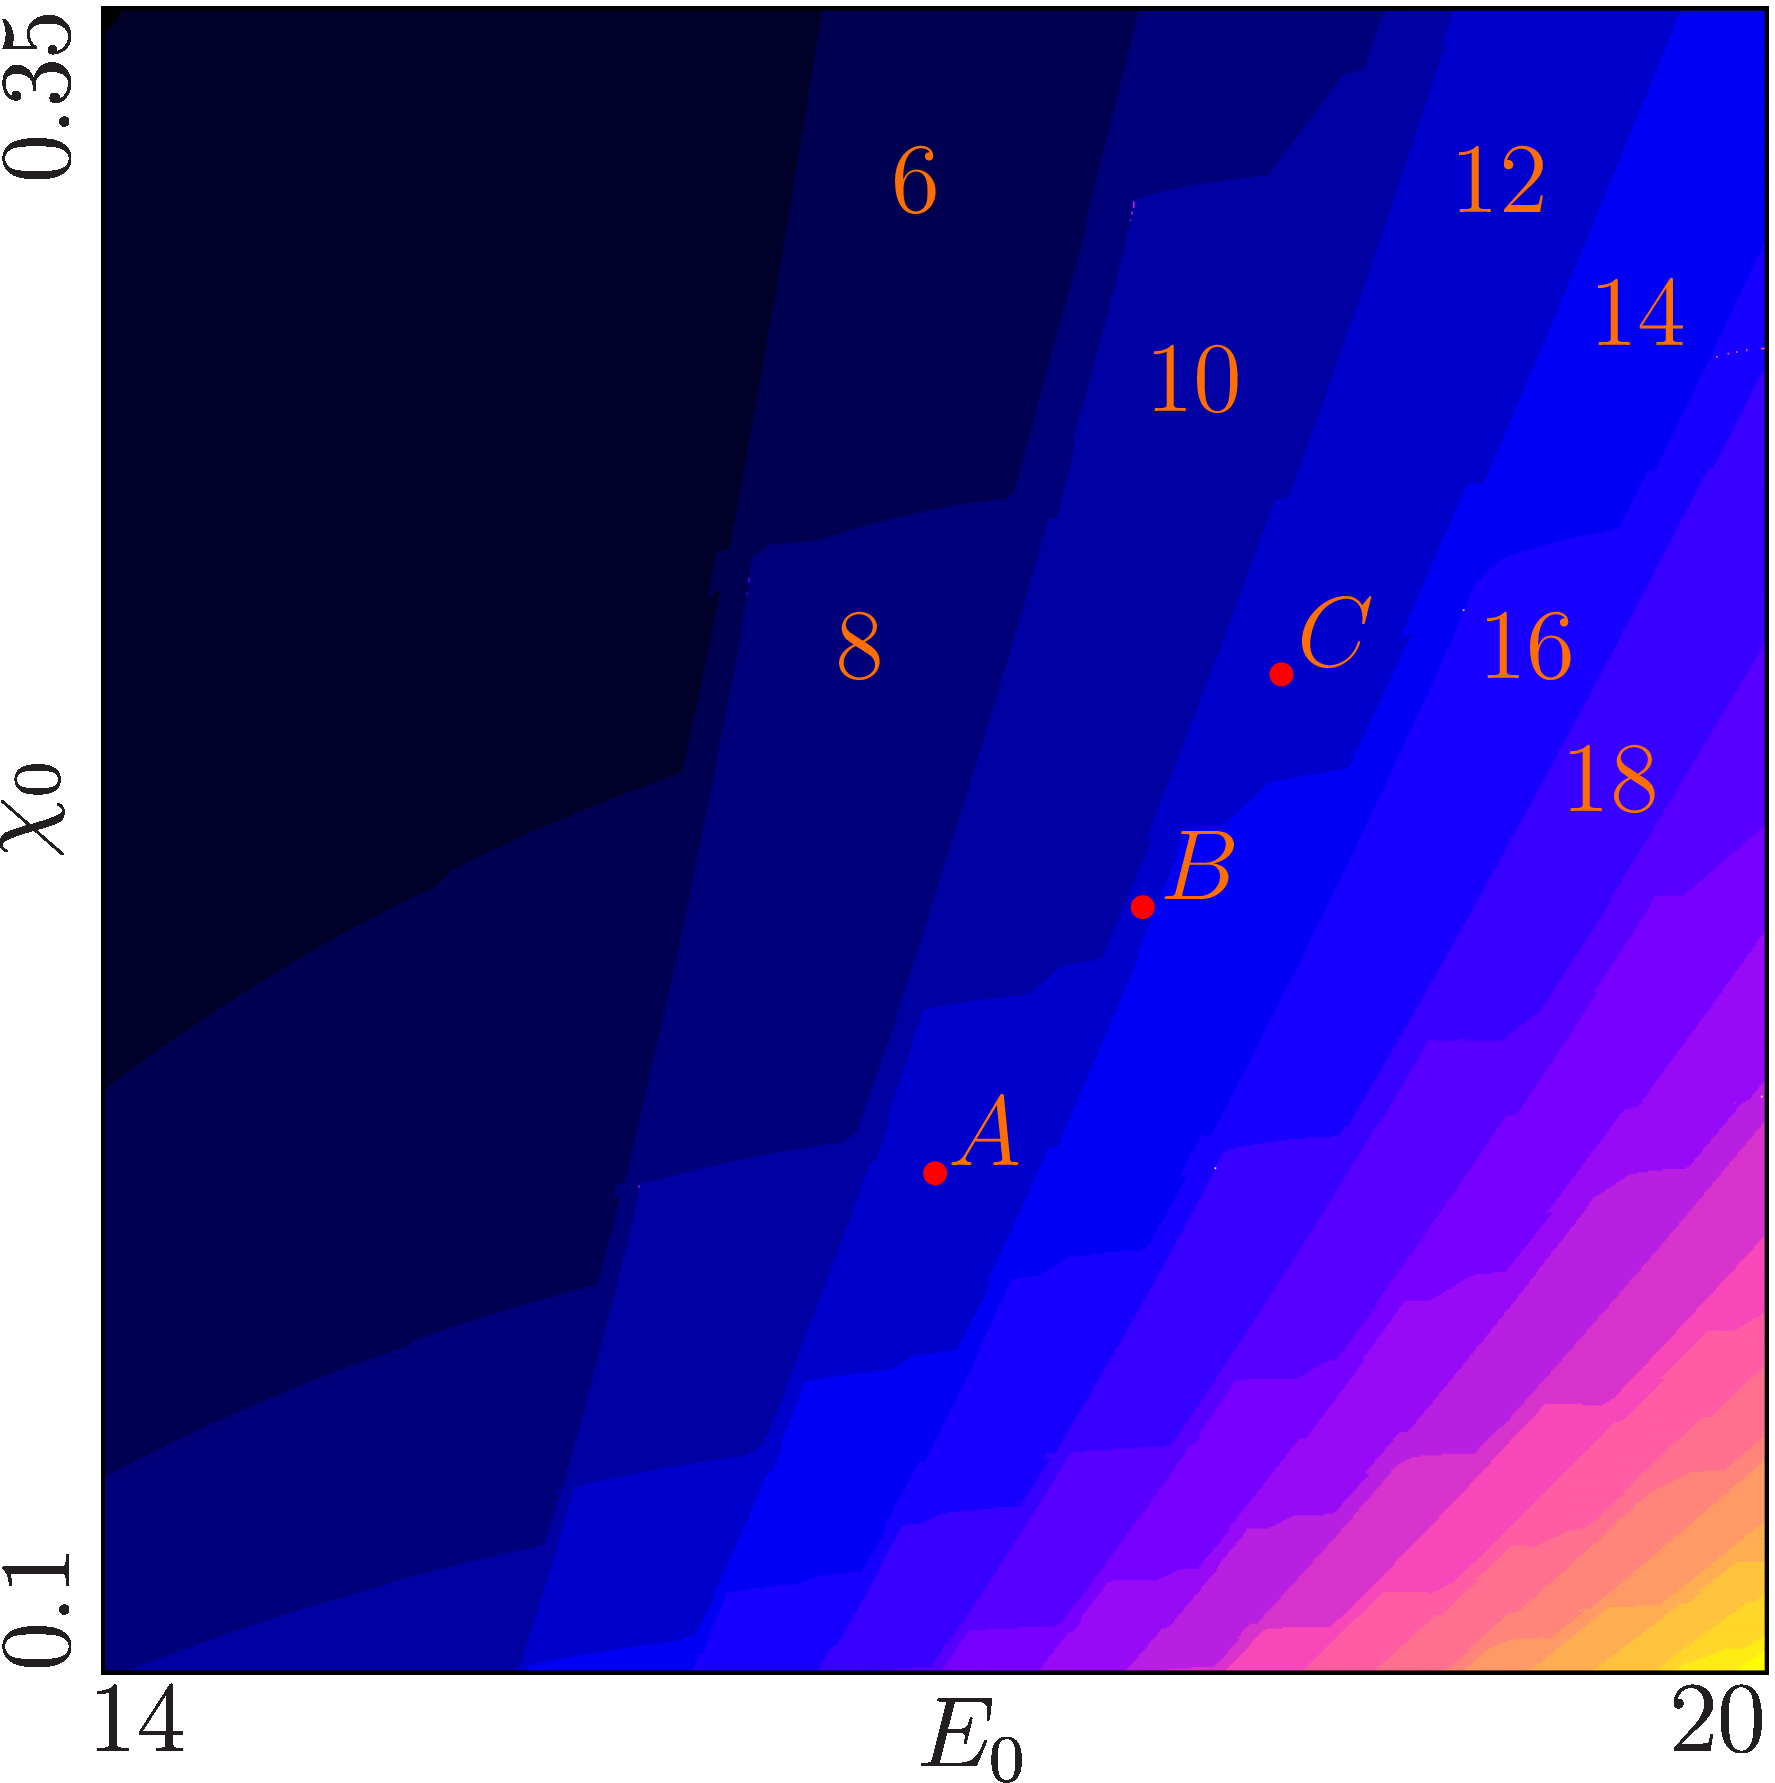
\includegraphics[width=0.4 \textwidth]{Figs/og_model_period.png}
			}{Original model}
			\qquad
			\stackunder[5pt]{
				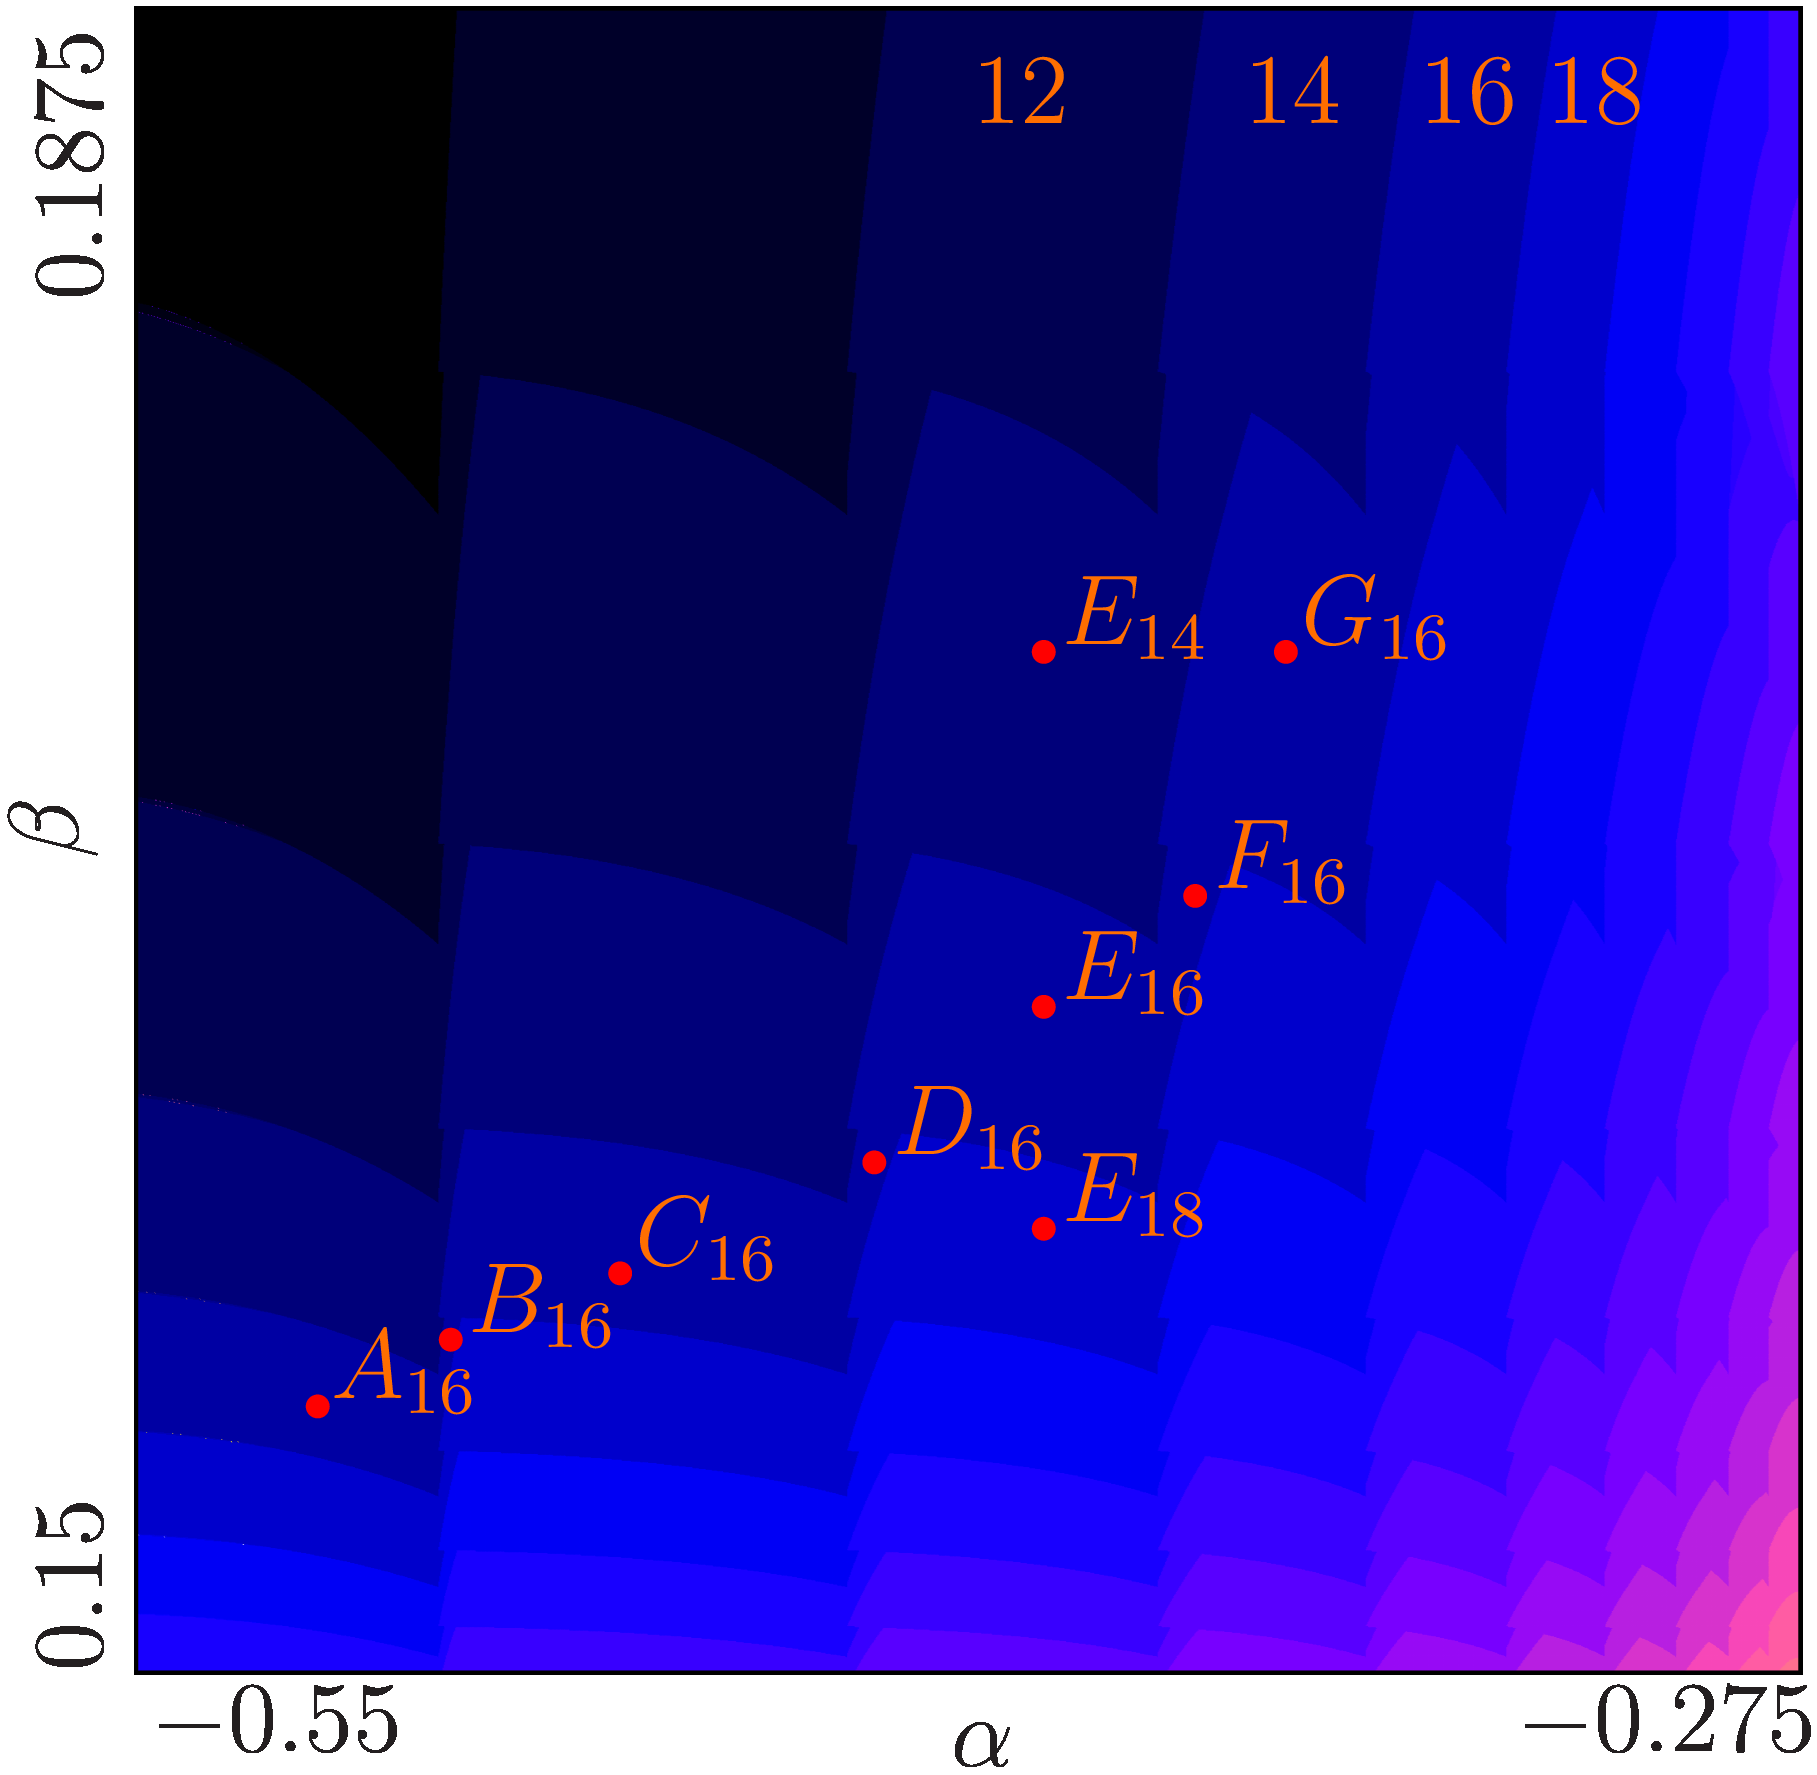
\includegraphics[width=0.41 \textwidth]{Figs/archetypal_model_period.png}
			}{Archetypal model}
		\end{figure}
	}
	\only<2>{
		\begin{figure}
			\centering
			\stackunder[5pt]{
				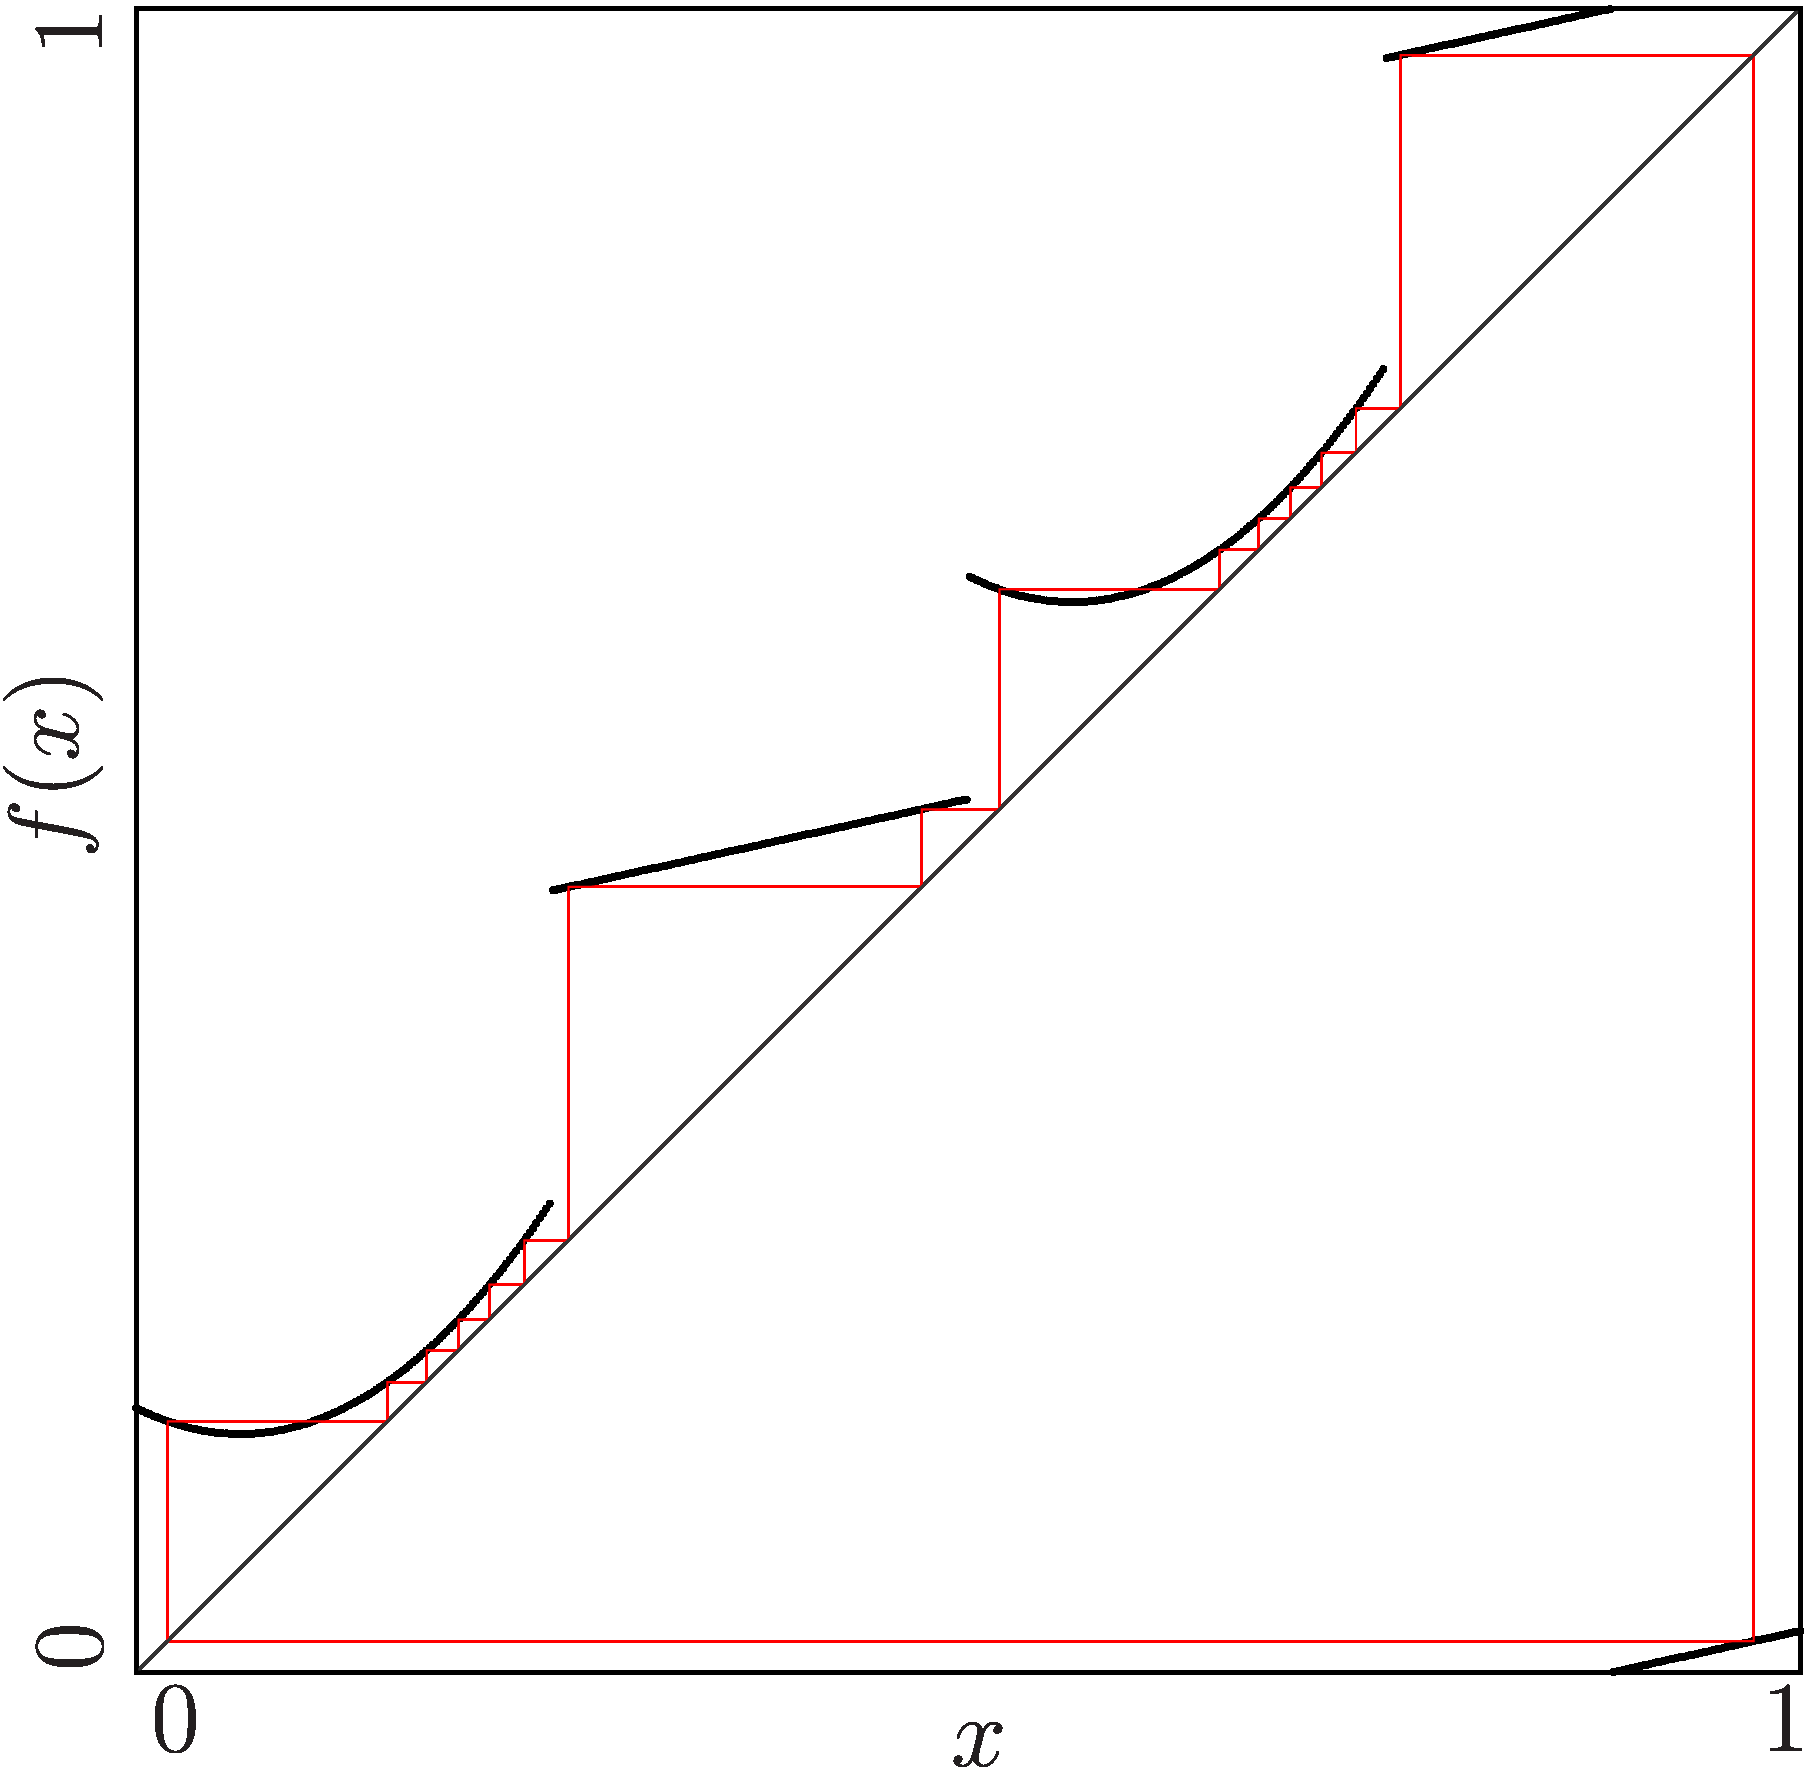
\includegraphics[width=0.3 \textwidth]{Figs/archetypal_model_cycle_c16.png}
			}{$C_{16}:\:\Cycle{\A^6\B^2\C^6\D^2}$}
			\stackunder[5pt]{
				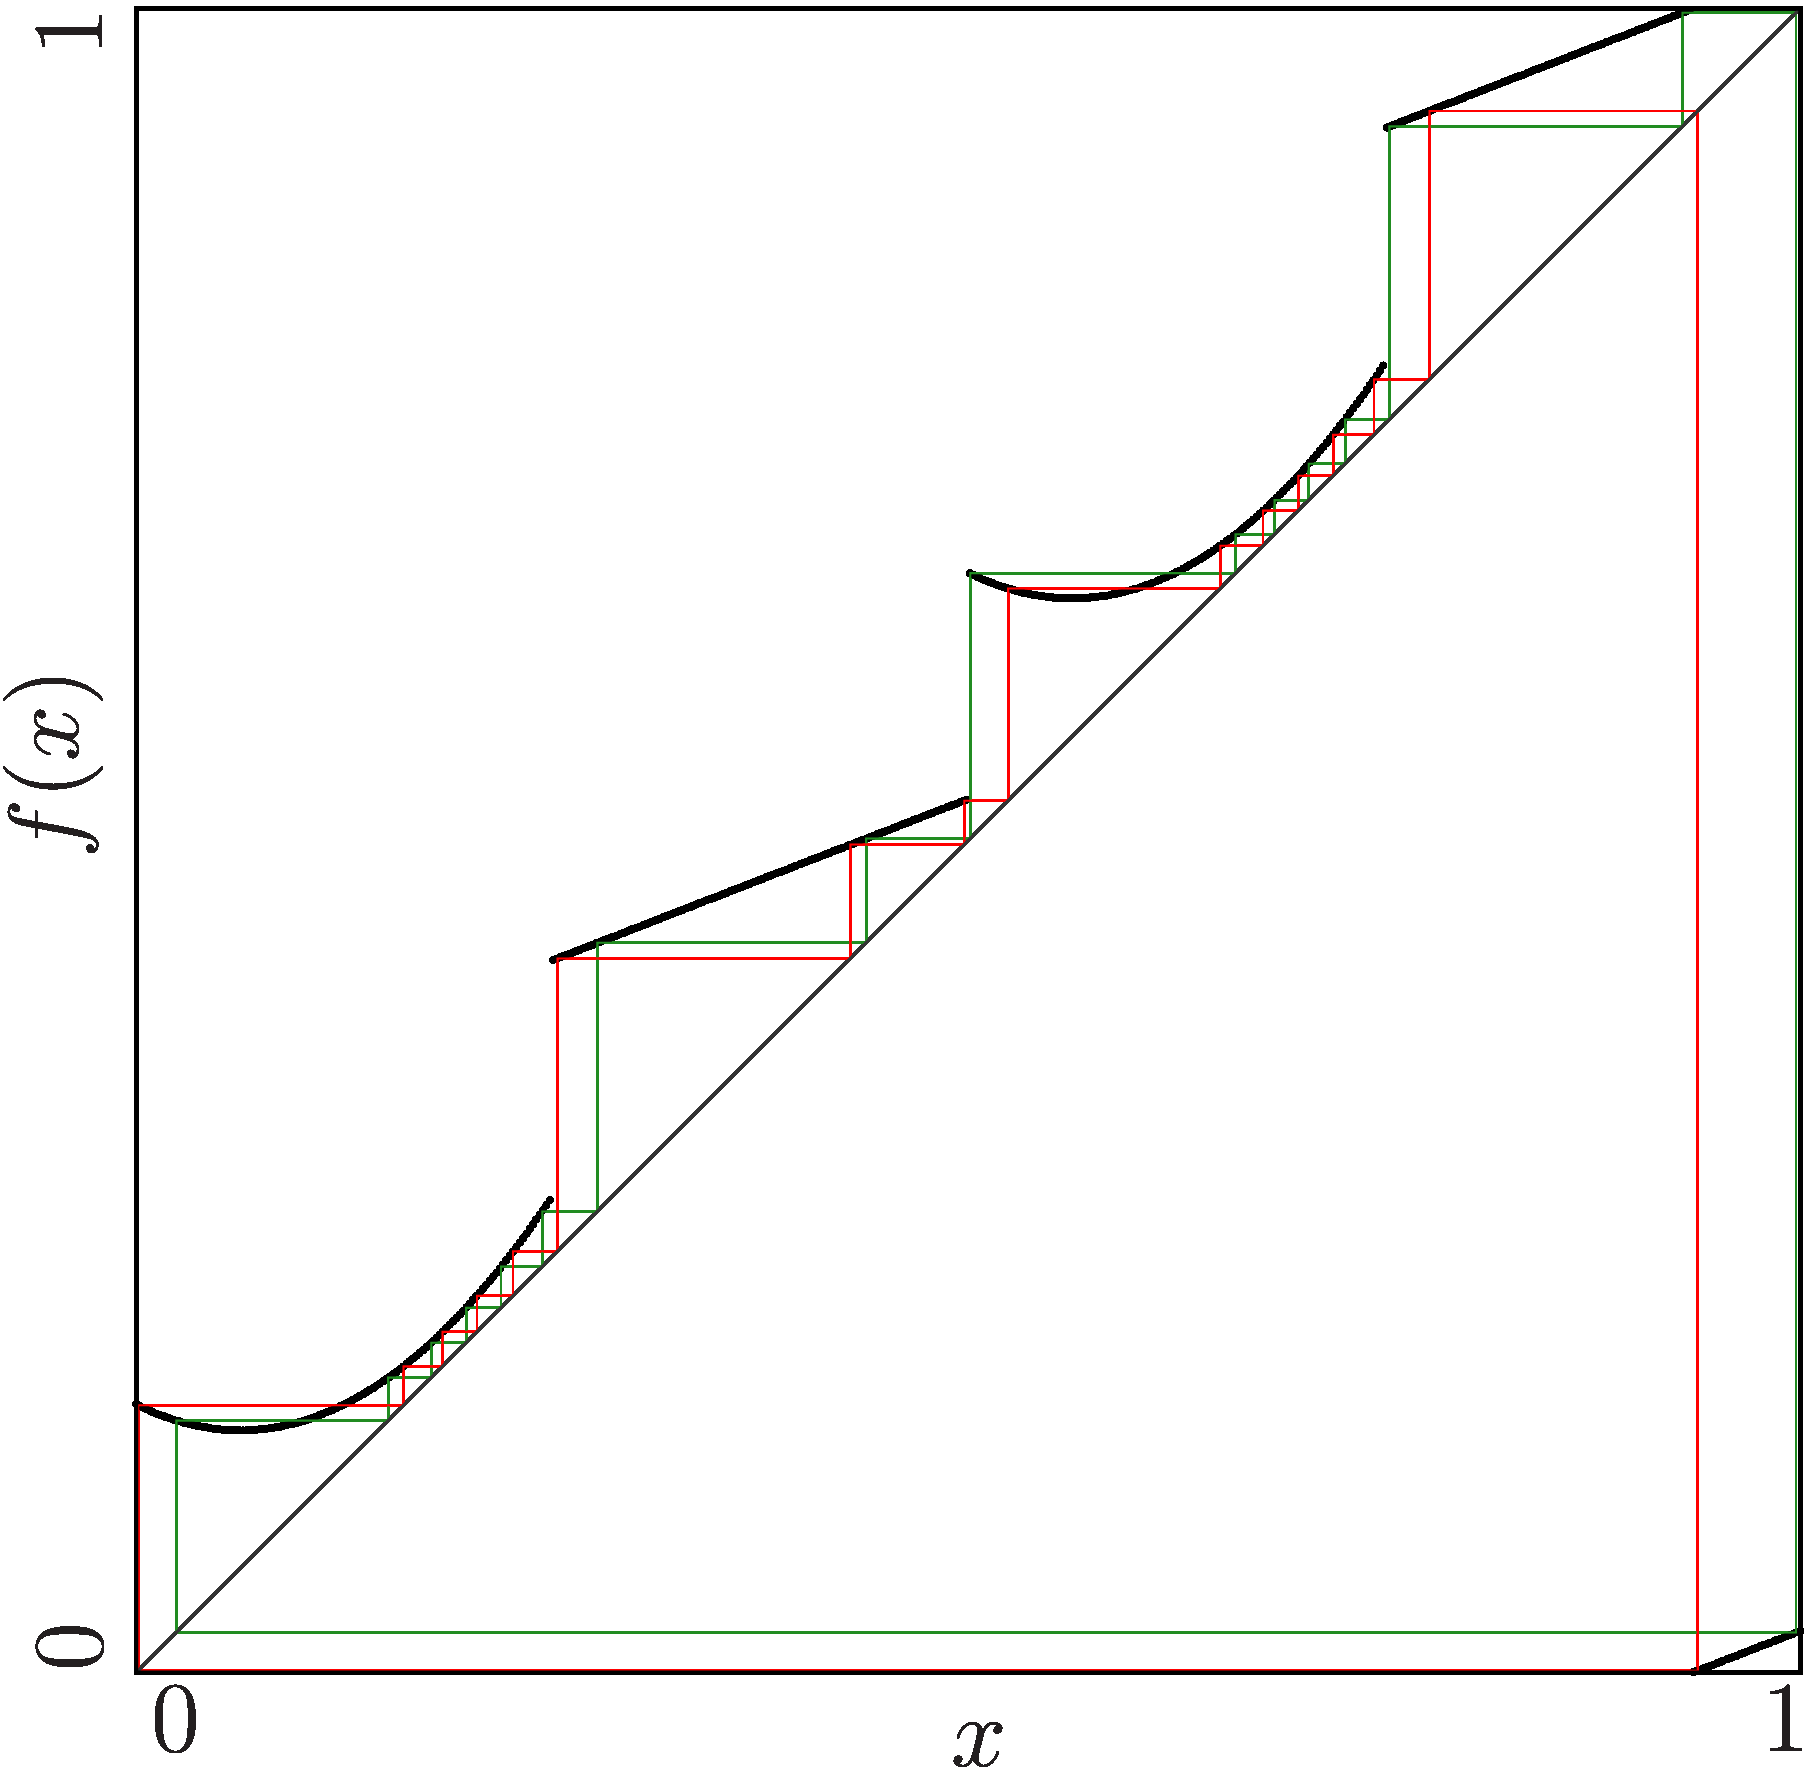
\includegraphics[width=0.3 \textwidth]{Figs/archetypal_model_cycle_d16.png}
			}{$D_{16}:\:\Cycle{\A^6\B^2\C^5\D^3},\Cycle{\A^5\B^3\C^6\D^2}$}
			\stackunder[5pt]{
				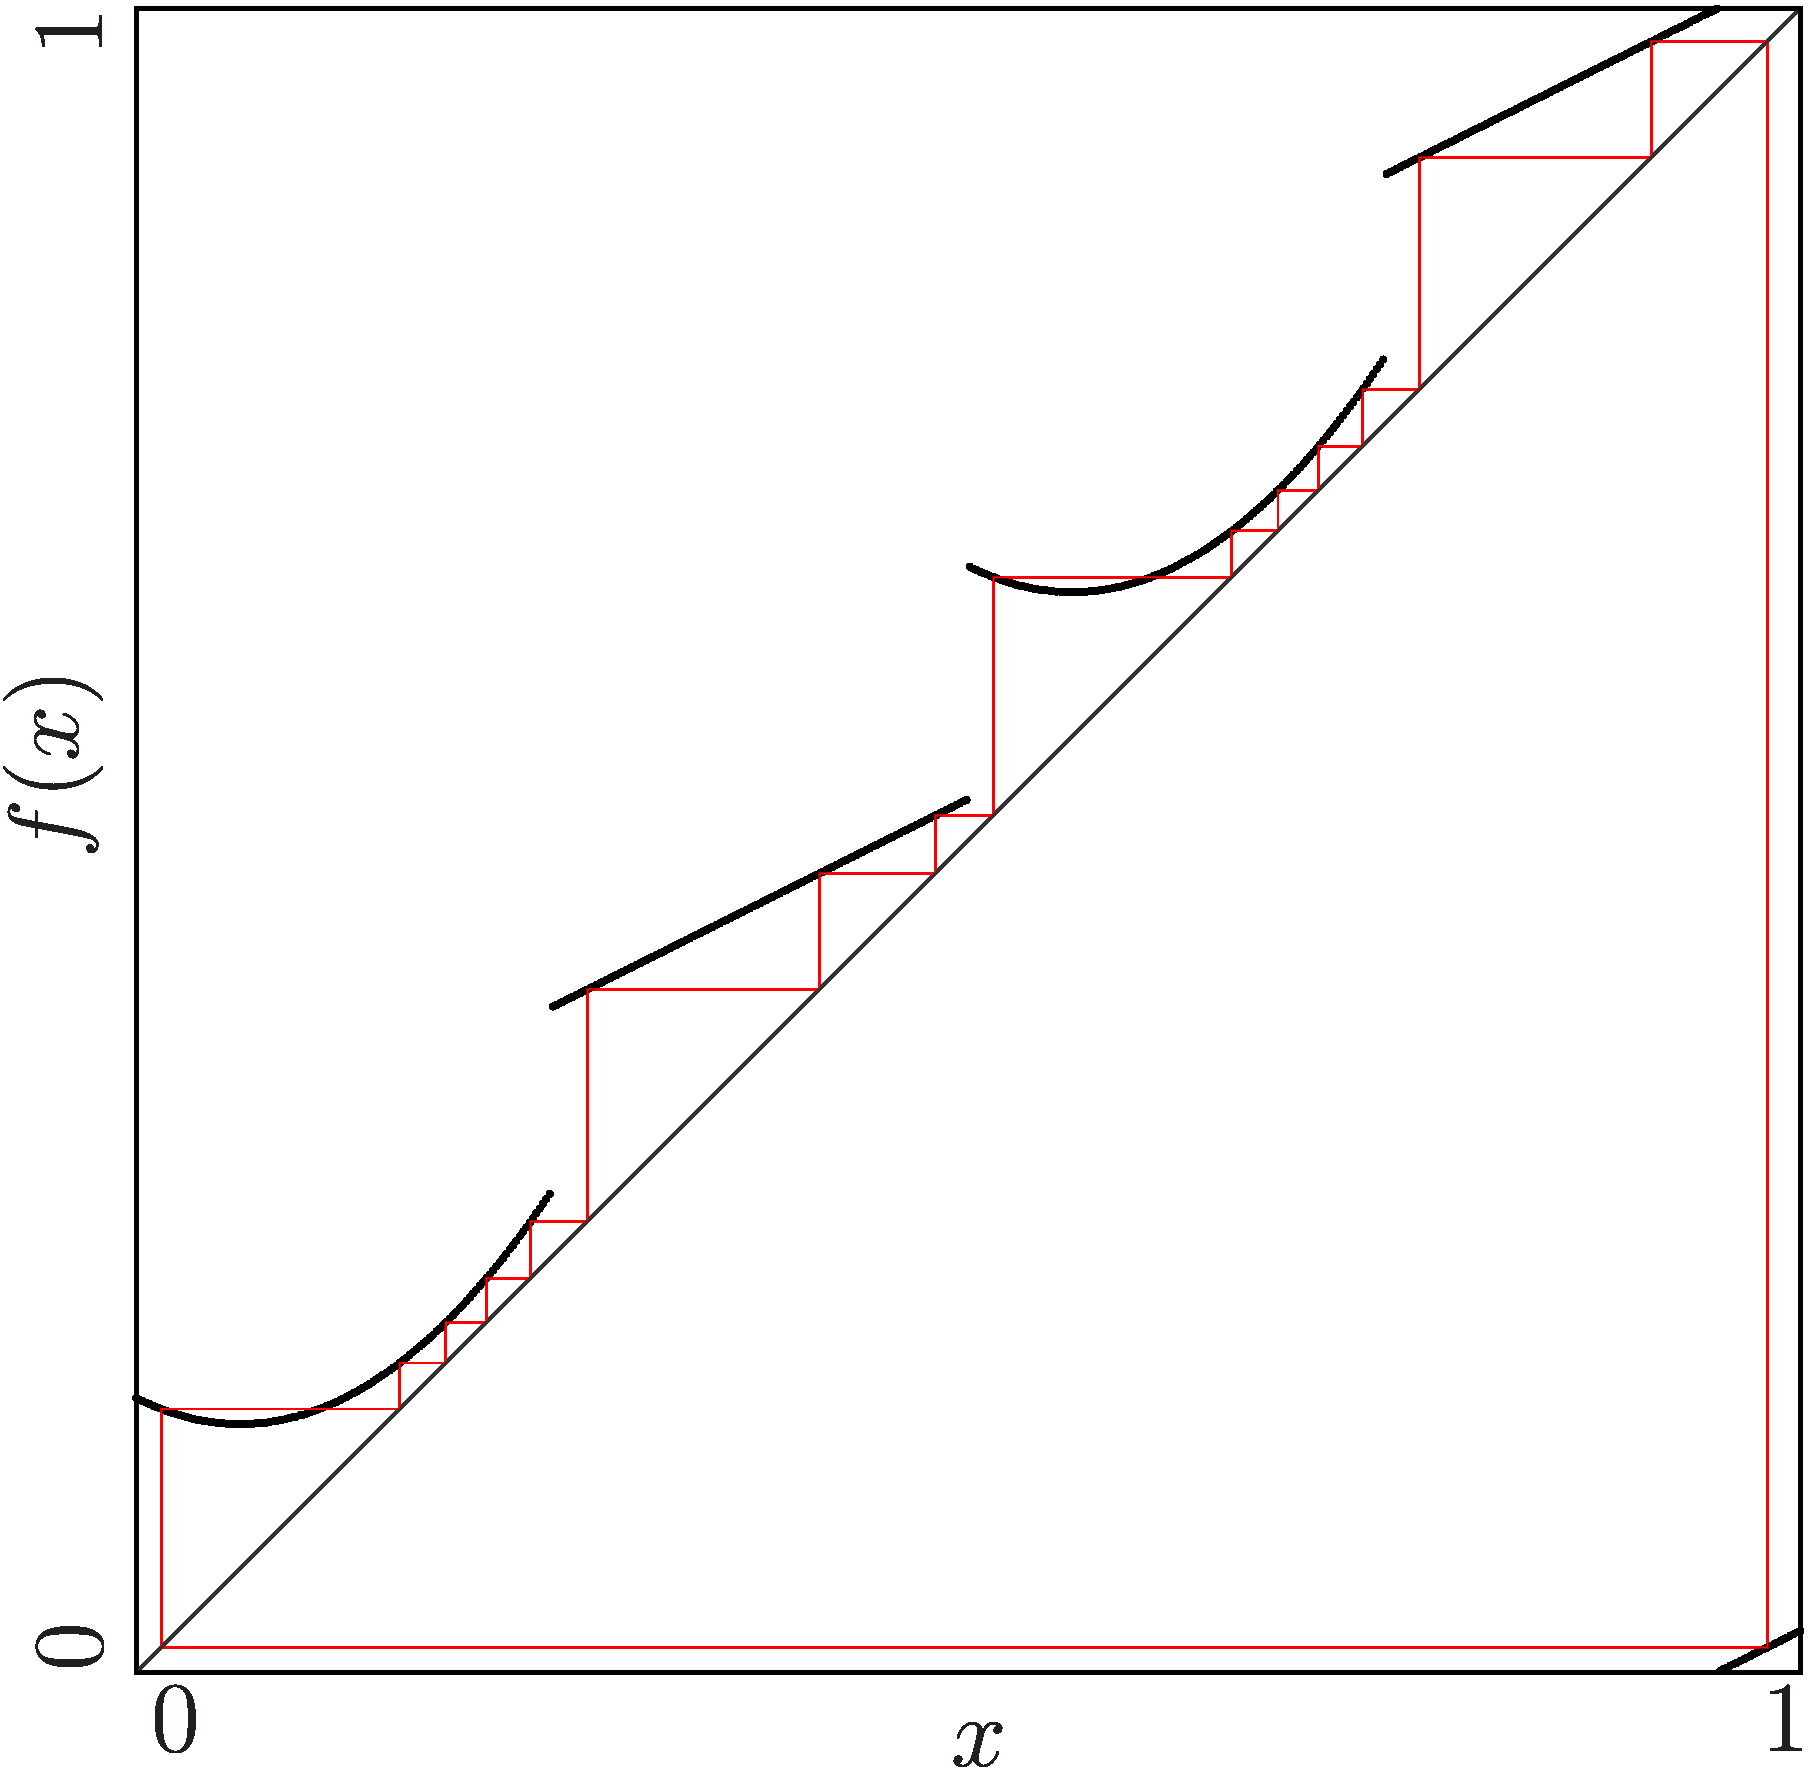
\includegraphics[width=0.3 \textwidth]{Figs/archetypal_model_cycle_e16.png}
			}{$E_{16}:\:\Cycle{\A^5\B^3\C^5\D^3}$}
		\end{figure}
	}
\end{frame}

\begin{frame}{Archetypal Model Equations}
	\vspace{-1.0em}
	\only<1>{
		\begin{align*}
			x_{n+1} = f(x_n) \mod 1
		\end{align*}
		\begin{align*}
			f(x) & = \begin{cases}
				         g(x)                                        & \text{ if } x < \frac{1}{2} \\
				         g\left(x - \frac{1}{2}\right) + \frac{1}{2} & \text{ else}
			         \end{cases}
		\end{align*}
		\begin{align*}
			g(x) & = \begin{cases}
				         g_L(x) = a_L \cdot x^2 + b_L \cdot x + c_L & \text{ if } x < \frac{1}{4} \\
				         g_R(x) = b_R \cdot x + c_R                 & \text{ else}
			         \end{cases}
		\end{align*}
	}
	\only<2>{
		\begin{columns}
			\begin{column}{.7 \textwidth}
				Fixed parameters:
				\begin{align*}
					a_L = 4 \text{ and } b_L = -\tfrac{1}{2}
				\end{align*}
				Variable parameters
				\begin{align*}
					 & c_L, b_R, c_R                                                                                                              \\
					\text{where} \qquad
					 & c_L = \beta,                                                                                                               \\
					 & b_R = -4 \cdot g_R\left(\tfrac{1}{4}\right) + 4 \cdot g_R\left(\tfrac{1}{2}\right),                                        \\
					 & c_R = 2 \cdot g_R\left(\tfrac{1}{4}\right) - 1 \cdot g_R\left(\tfrac{1}{2}\right),                                         \\[1em]
					\text{and} \qquad
					 & g_R\left(\tfrac{1}{4}\right) = \alpha, \text{and } g_R\left(\tfrac{1}{2}\right) = \tfrac{1}{2} + \epsilon \text{ is fixed}
				\end{align*}
			\end{column}
			\begin{column}{.3 \textwidth}
				\begin{figure}
					\centering
					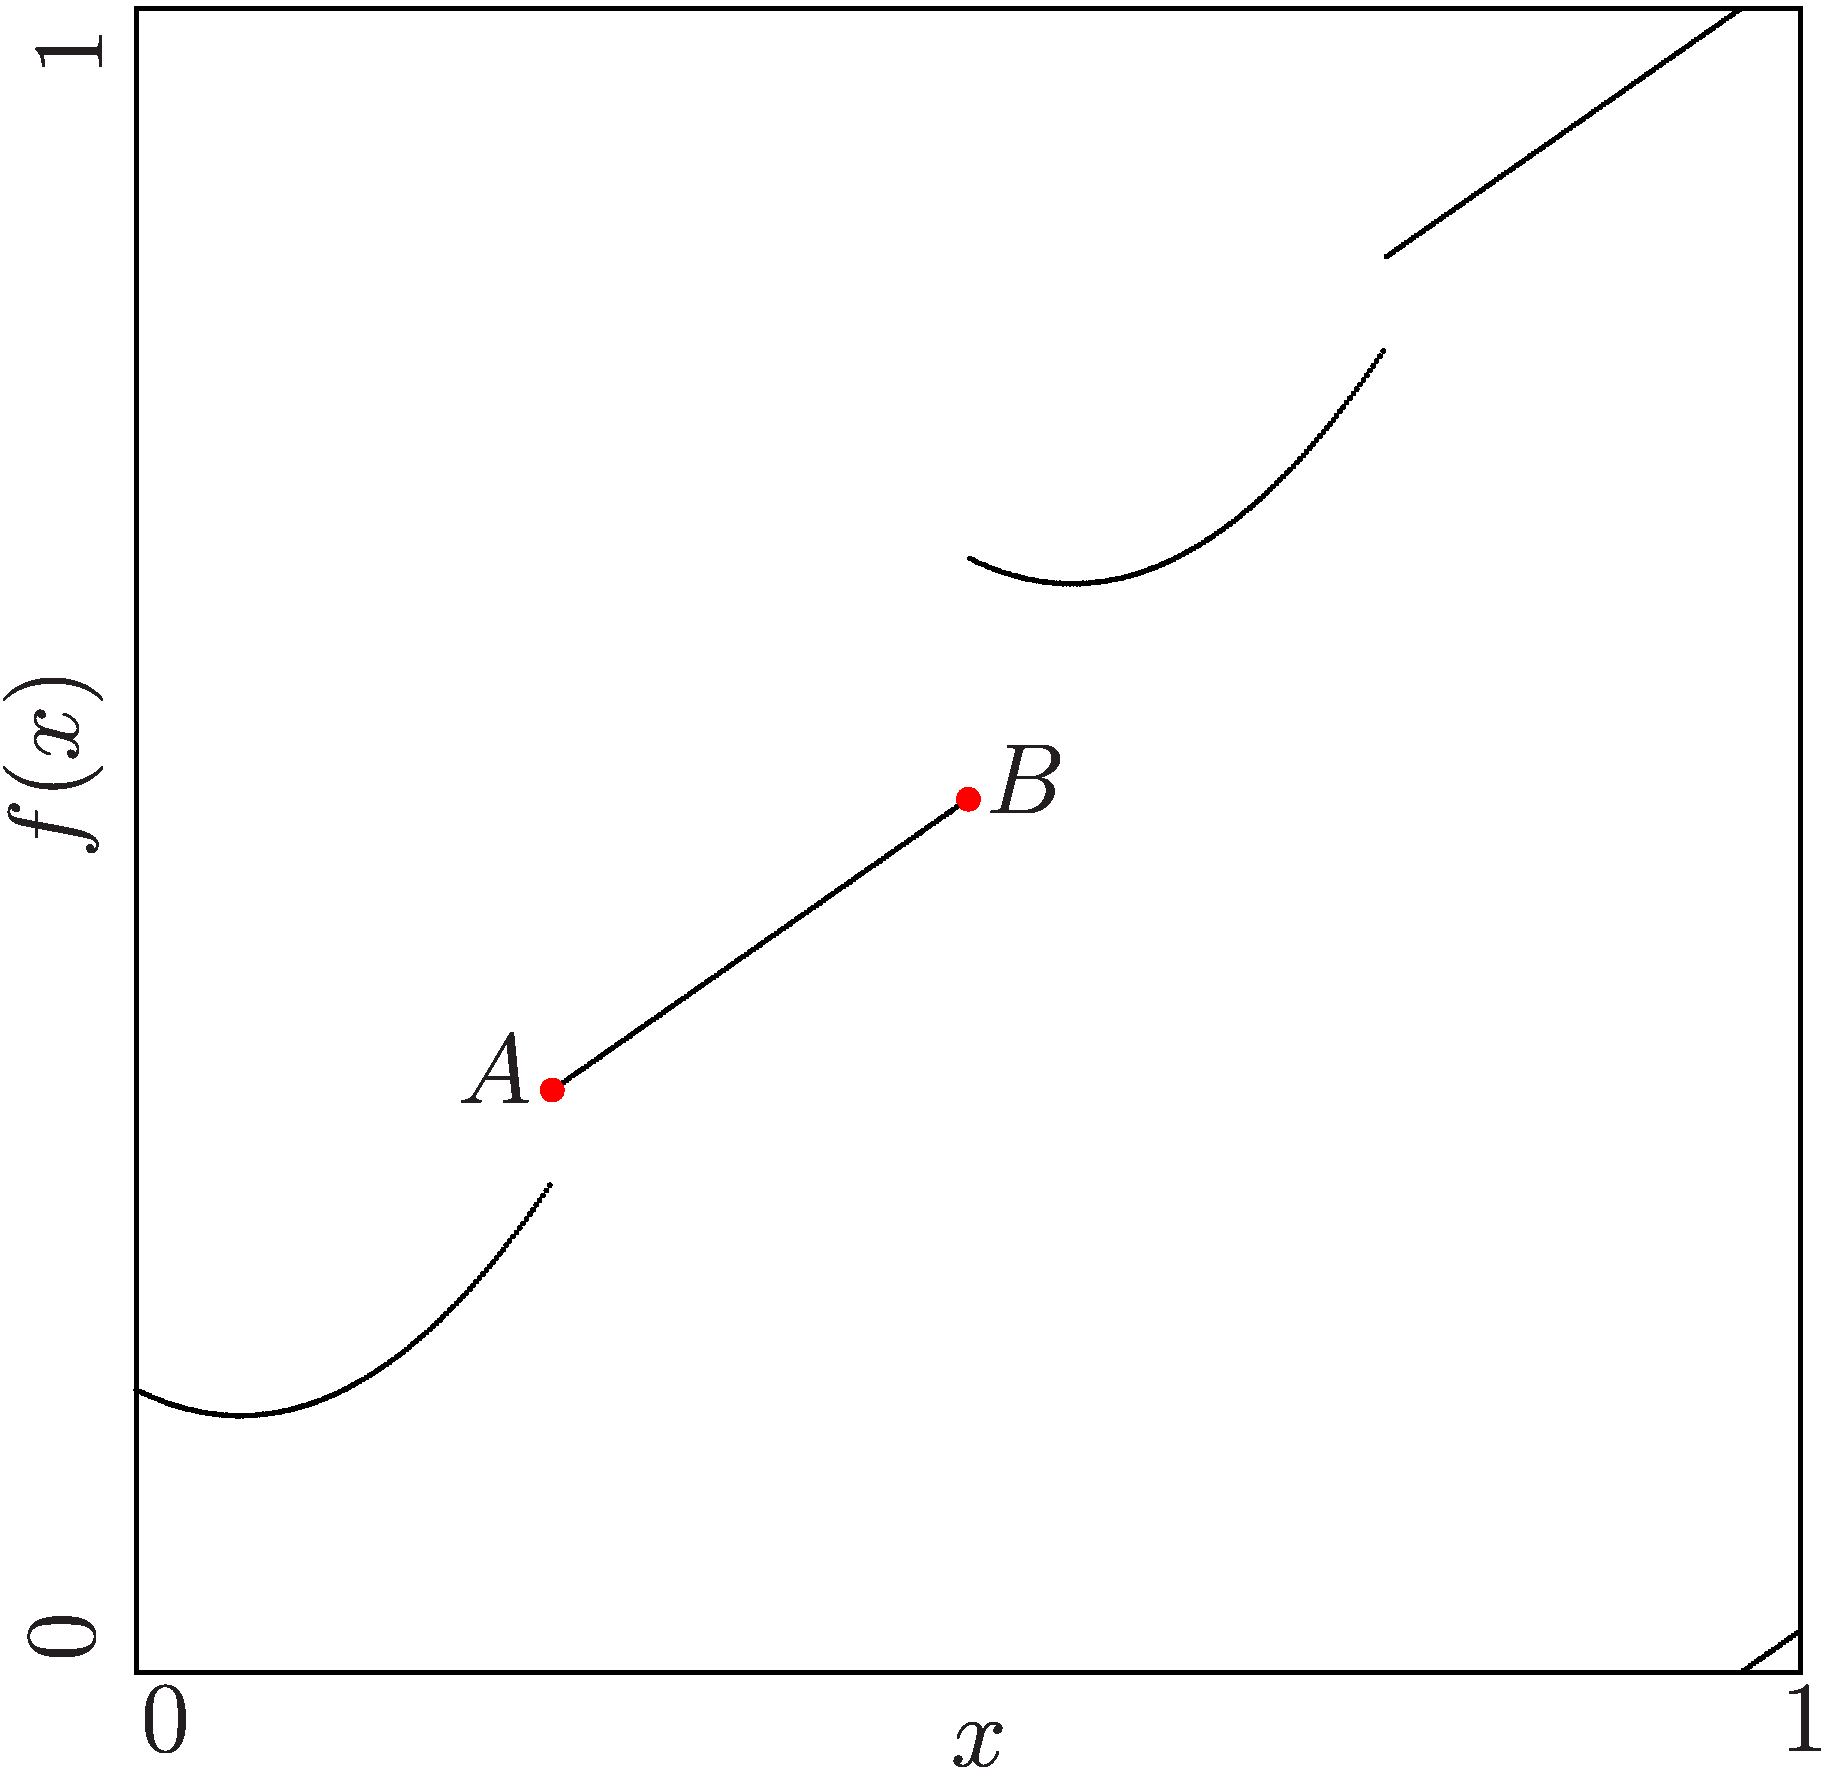
\includegraphics[height=.5 \textheight]{Figs/archetypal_model_parameter_effects_illustration.png}
				\end{figure}
			\end{column}
		\end{columns}
	}
\end{frame}

\begin{frame}{Archetypal Model Results}
	\begin{itemize}
		\item Description of the bifucation structure
		\item Explanation of coexisting cycles via the symmetry
		\item Explanation of double border collisions via the symmetry
		\item Discovery of 4 coexisting cycles not discovered in the original model
		      \begin{itemize}
			      \item Confirmation of 4 coexisting cycles in the original model
		      \end{itemize}
	\end{itemize}
\end{frame}

\begin{frame}{Period-Adding?}
	\vspace{-1em}
	\begin{itemize}
		\item Chains overlap
		\item What happens, when they no longer overlap?
		      \vspace{1em}
		\item Prediction: Period-Adding
		      %\item Turns up often
		      %\item E.g. Edge of main bubble of mandelbrot set
	\end{itemize}
	\begin{figure}
		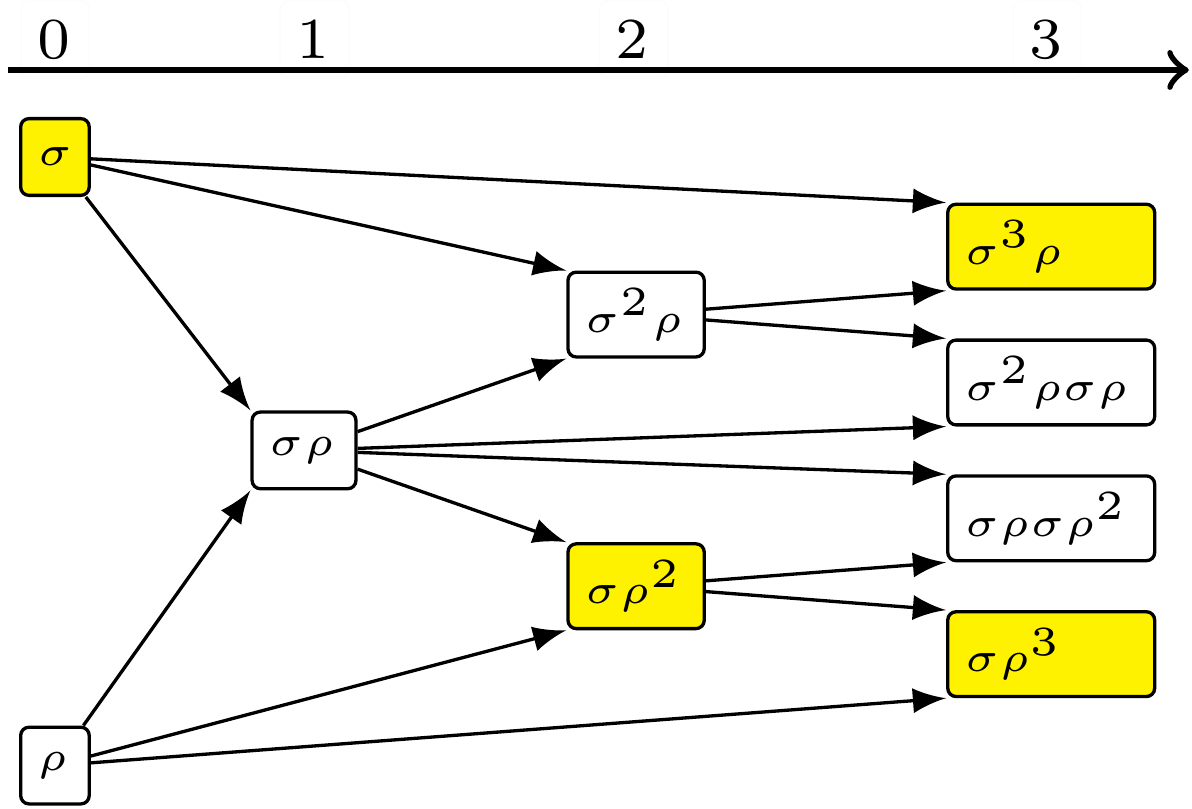
\includegraphics[height=.5 \textheight]{Figs/Trees/ClassicalAdding/adding.png}
	\end{figure}
\end{frame}

\begin{frame}{Archetypal Model with Different Parameters}
	\only<1>{
		\begin{figure}
			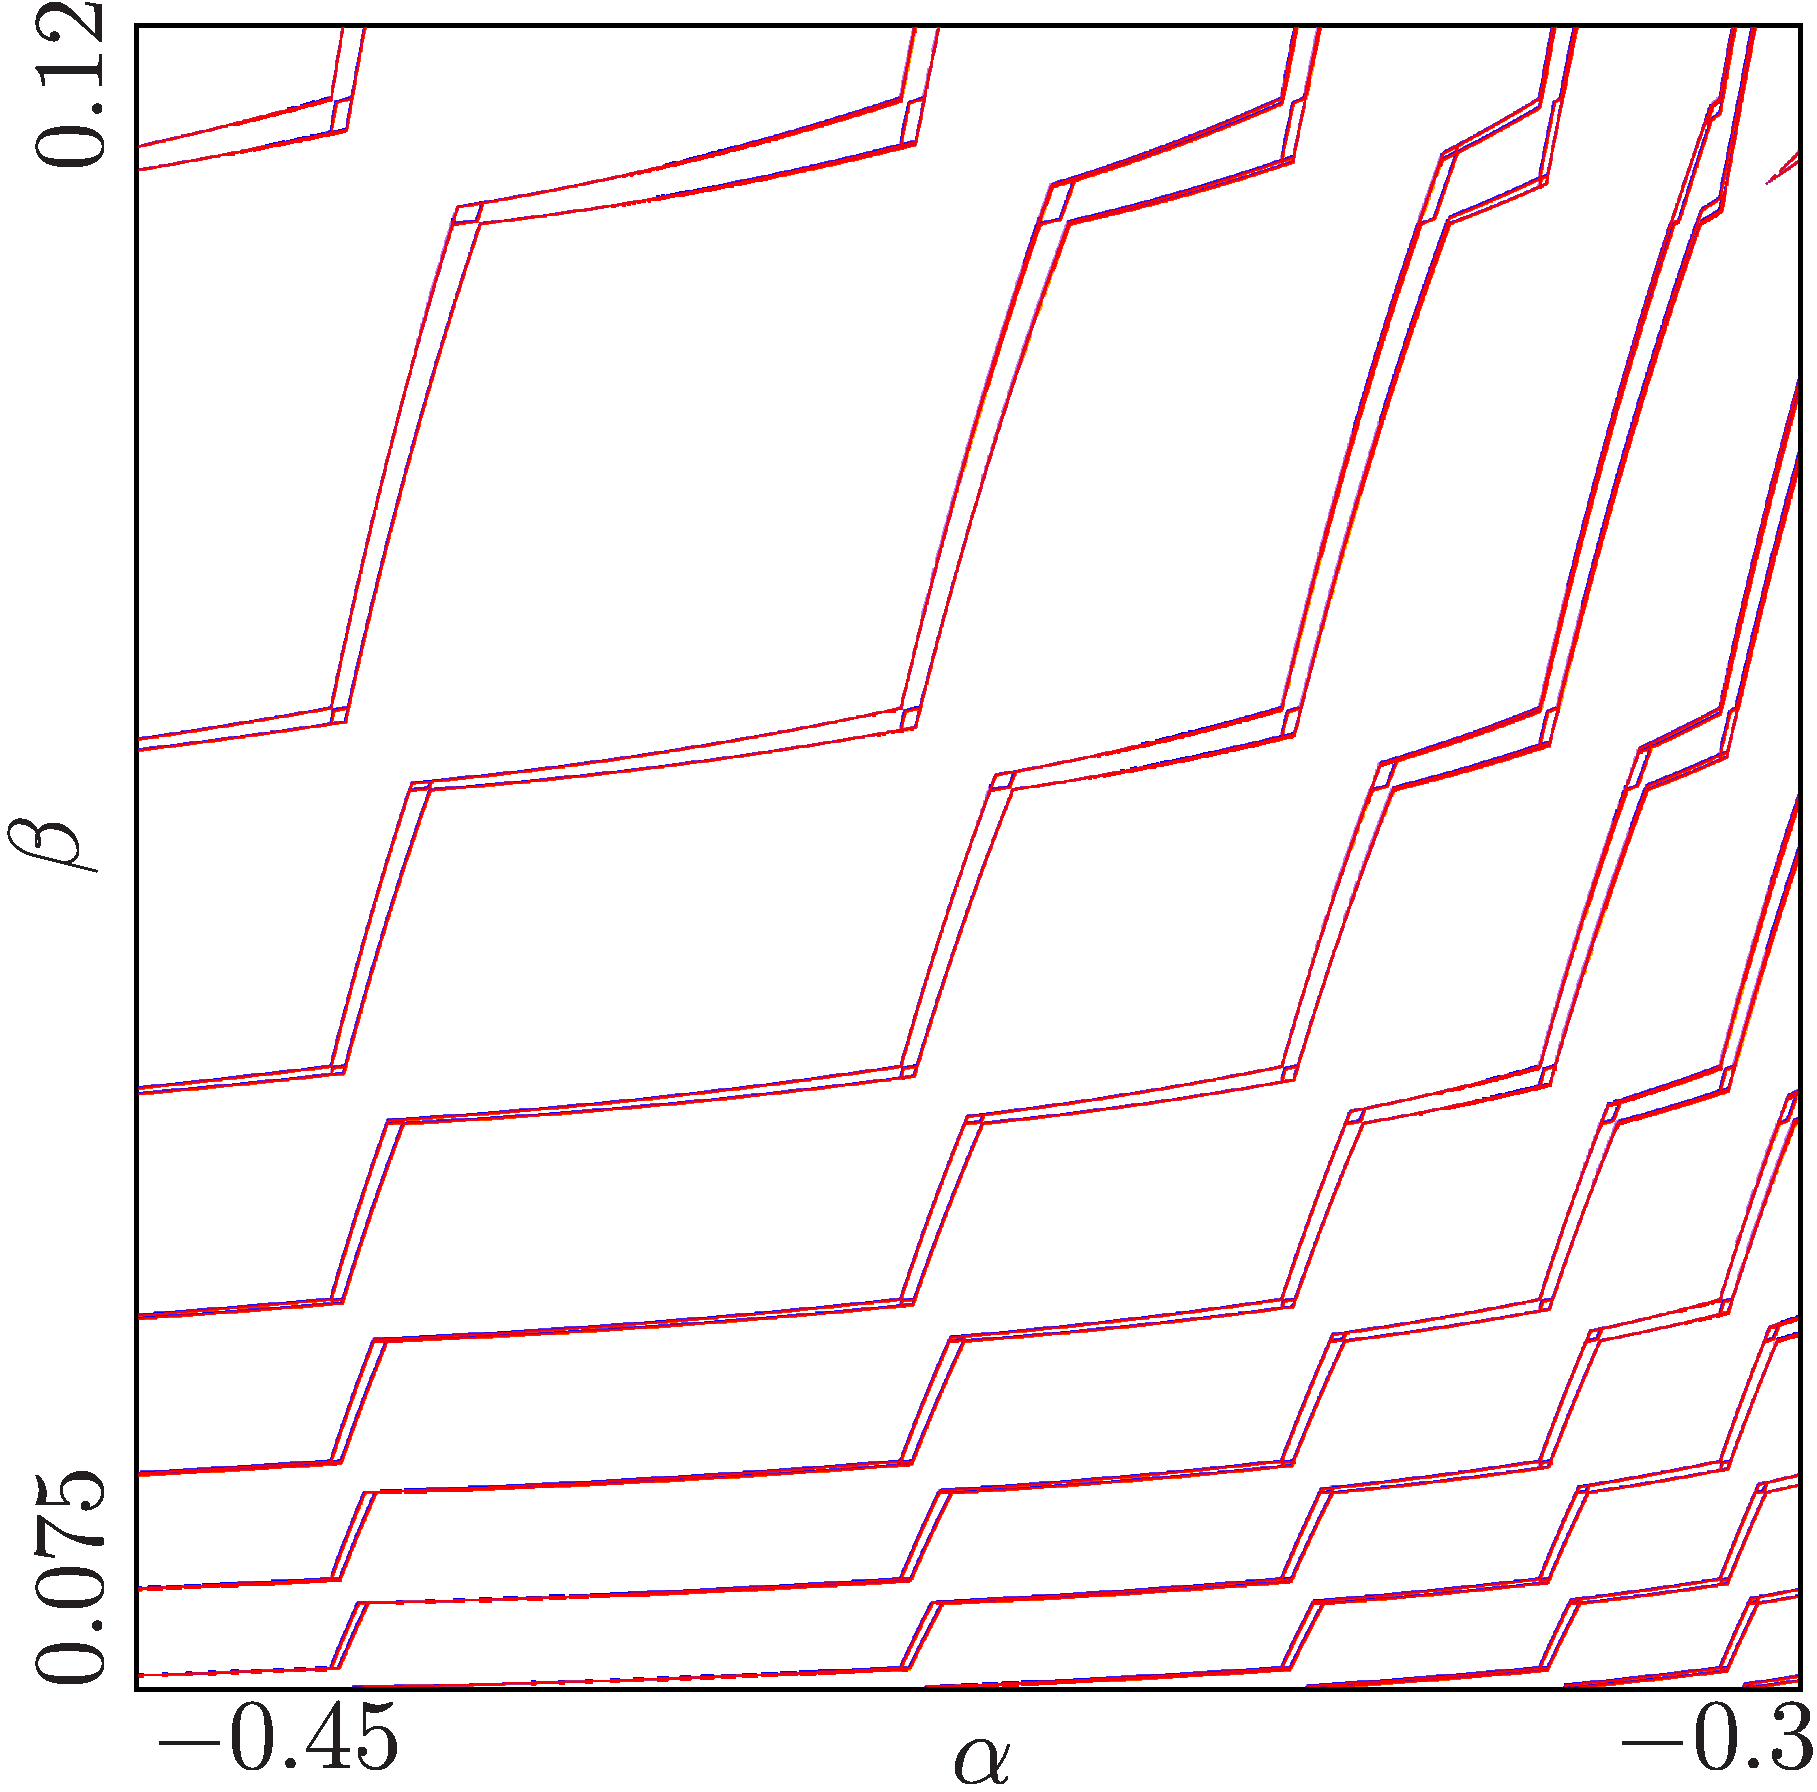
\includegraphics[width=.4 \textwidth]{Figs/archetypal_model_regions_drifting_apart.png}
			\quad
			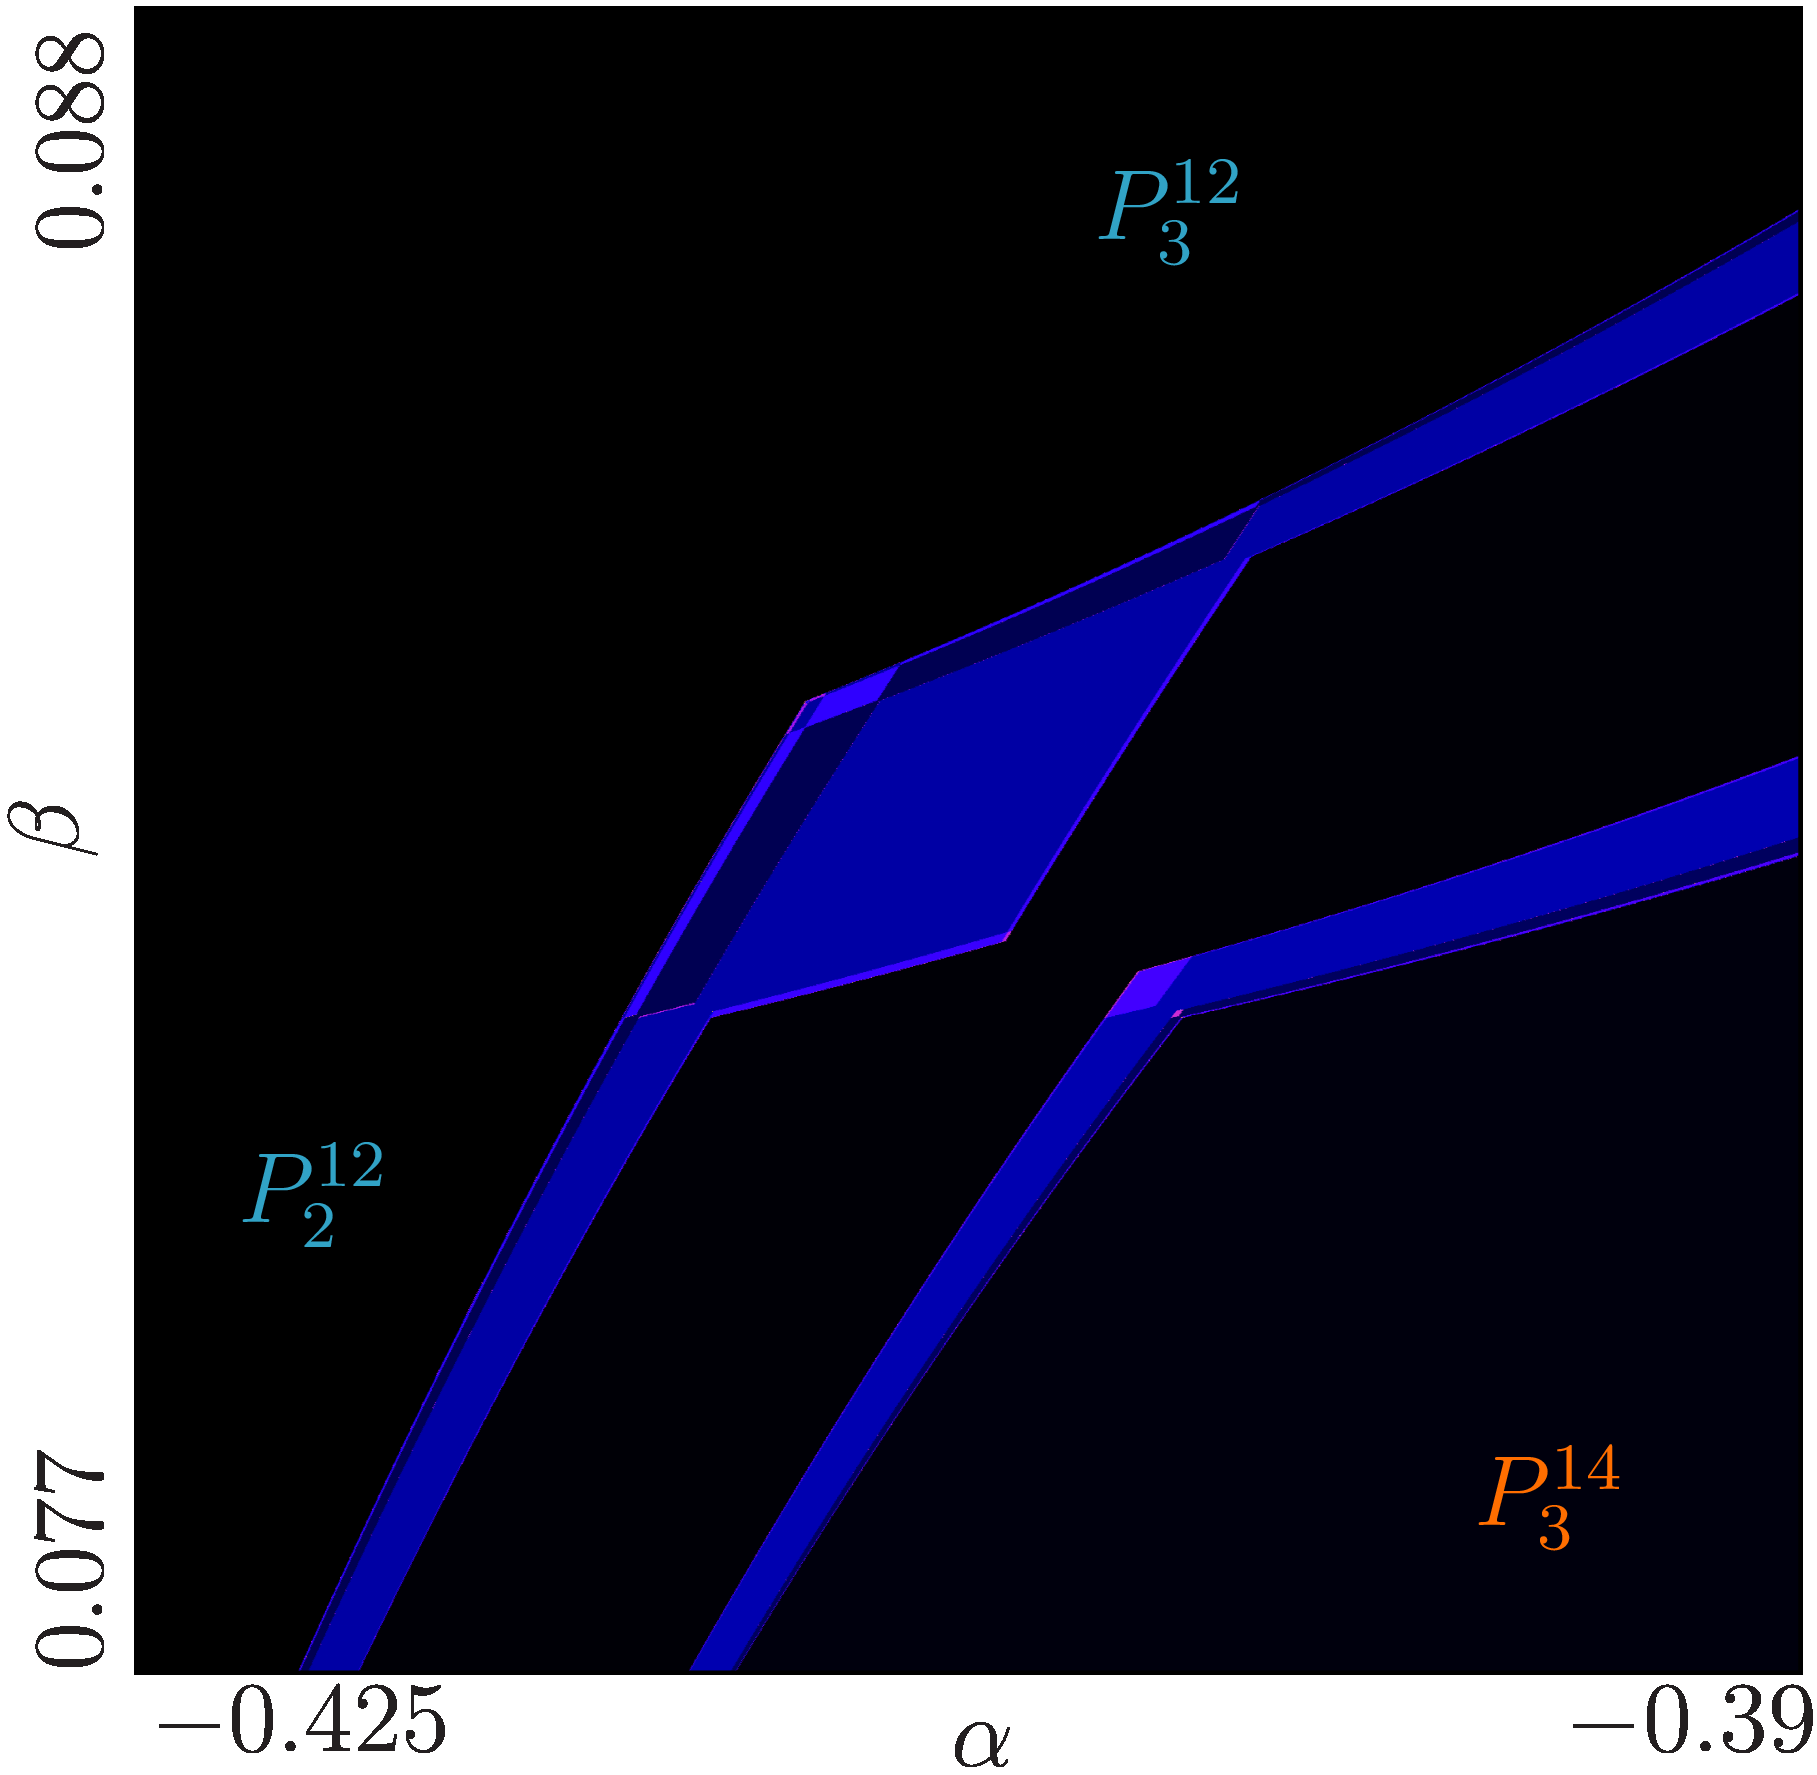
\includegraphics[width=.4 \textwidth]{Figs/archetypal_model_adding_like_period_corner.png}
		\end{figure}
	}
	\only<2>{
		\vspace{-1em}
		\begin{figure}
			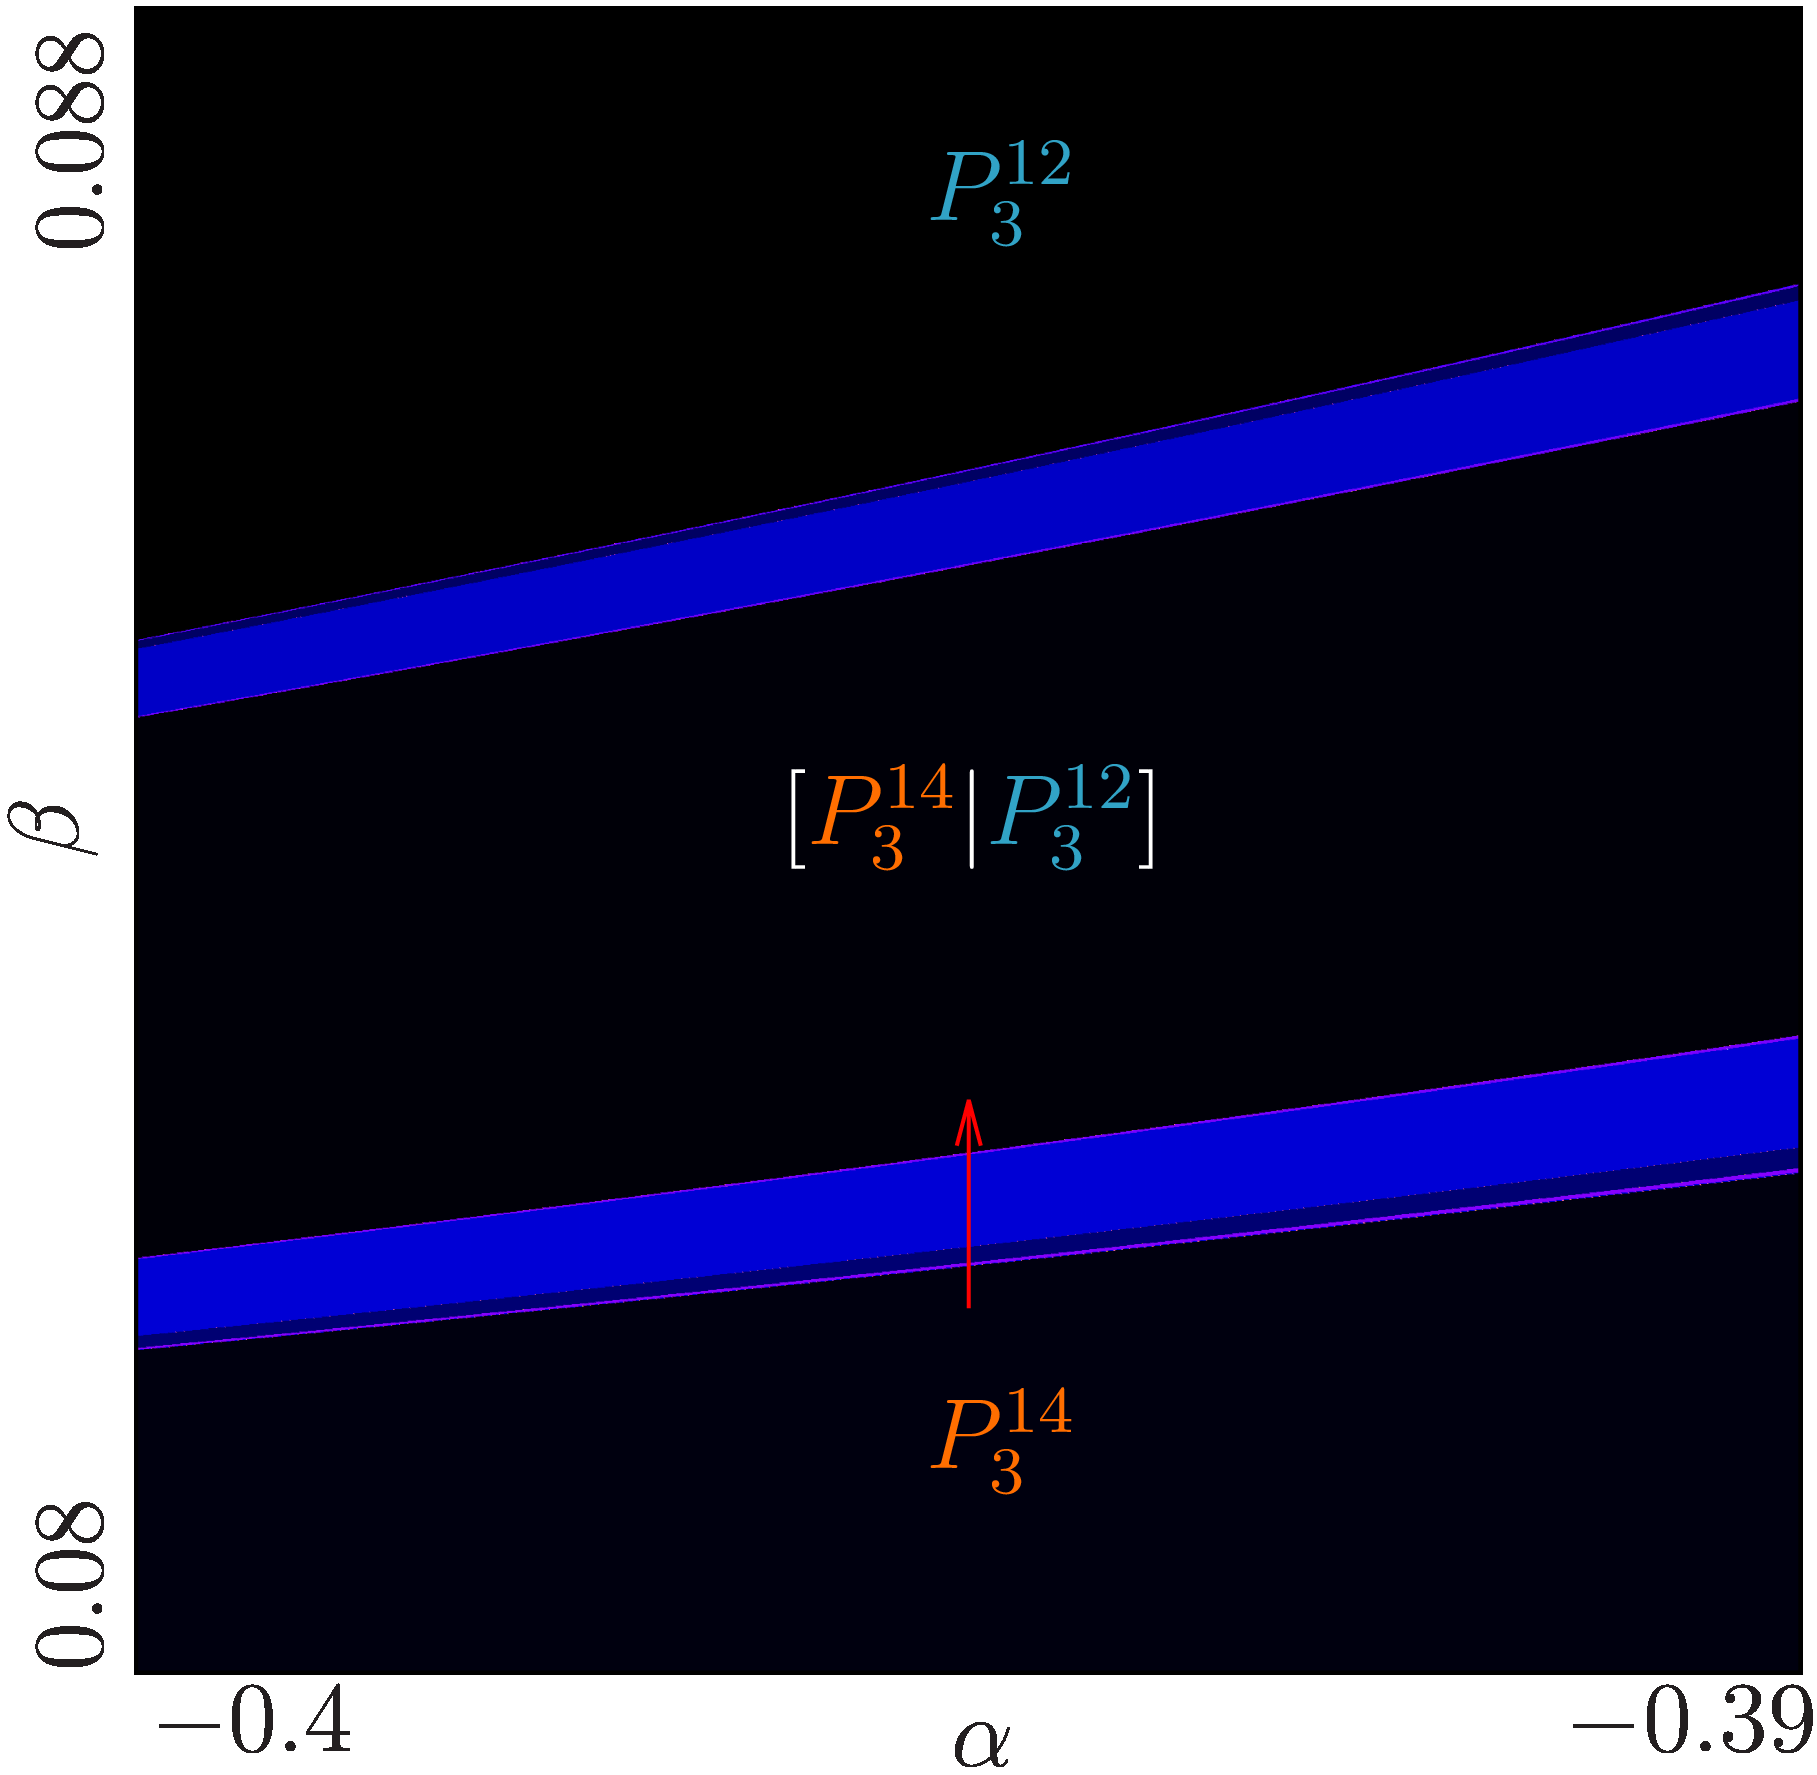
\includegraphics[width=.4 \textwidth]{Figs/archetypal_model_full_add_hor_2D.png}
			\qquad
			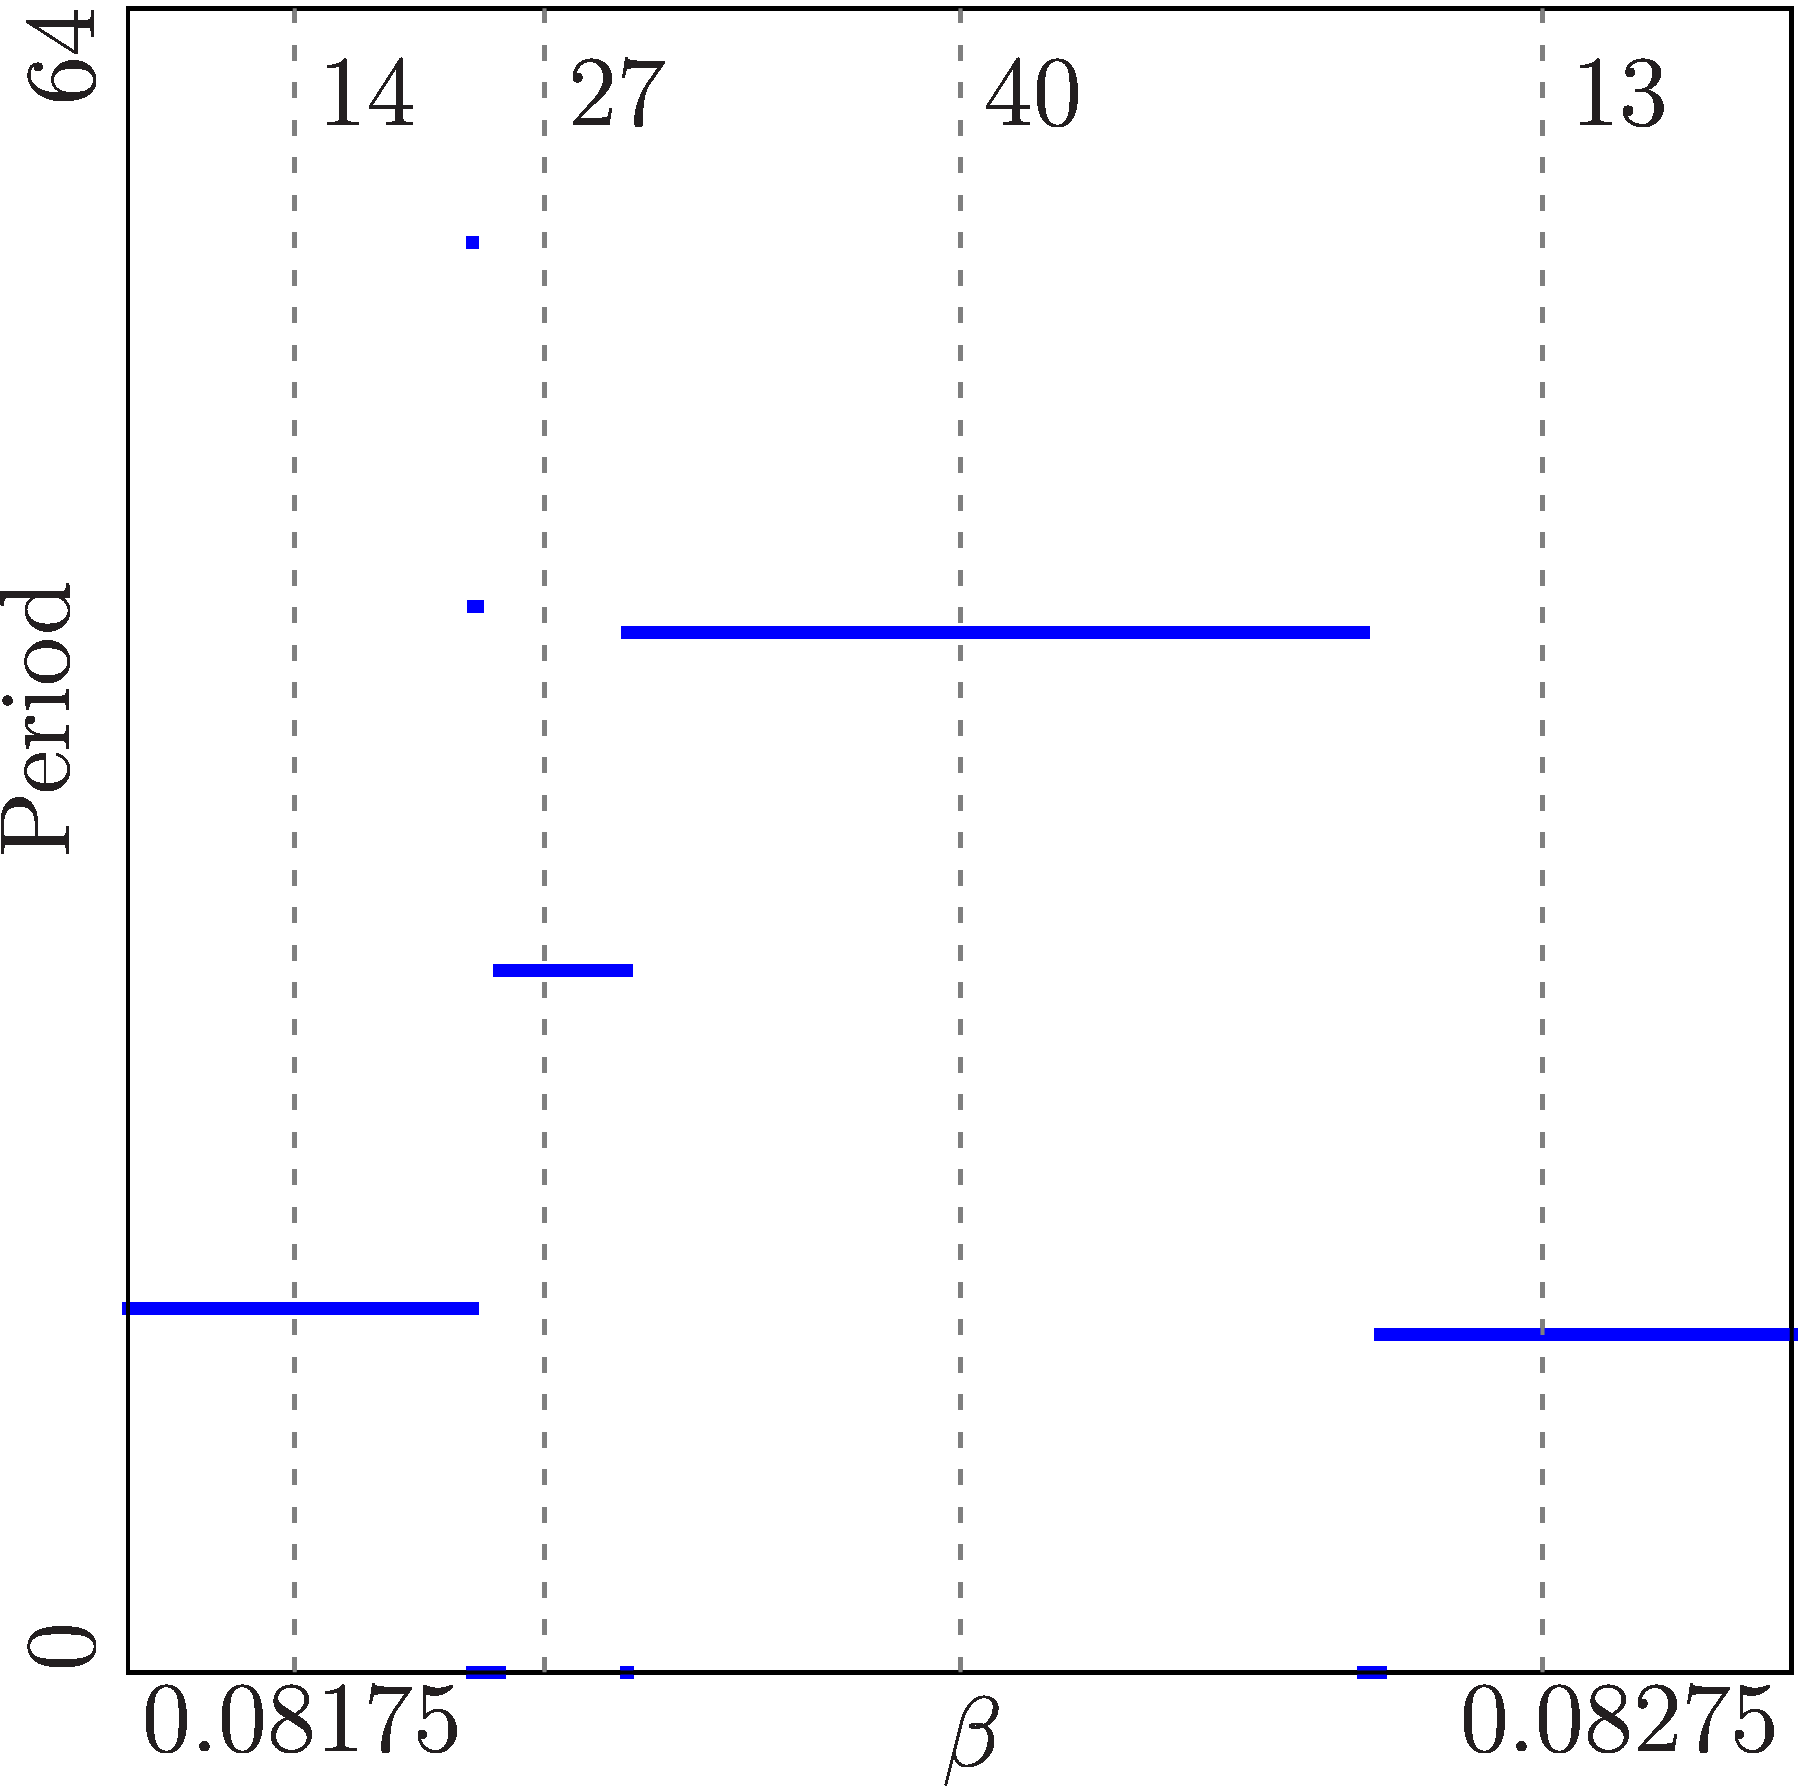
\includegraphics[width=.4 \textwidth]{Figs/archetypal_model_full_add_hor_1D.png}
		\end{figure}
	}
	\only<3>{
		\vspace{-1em}
		\begin{figure}
			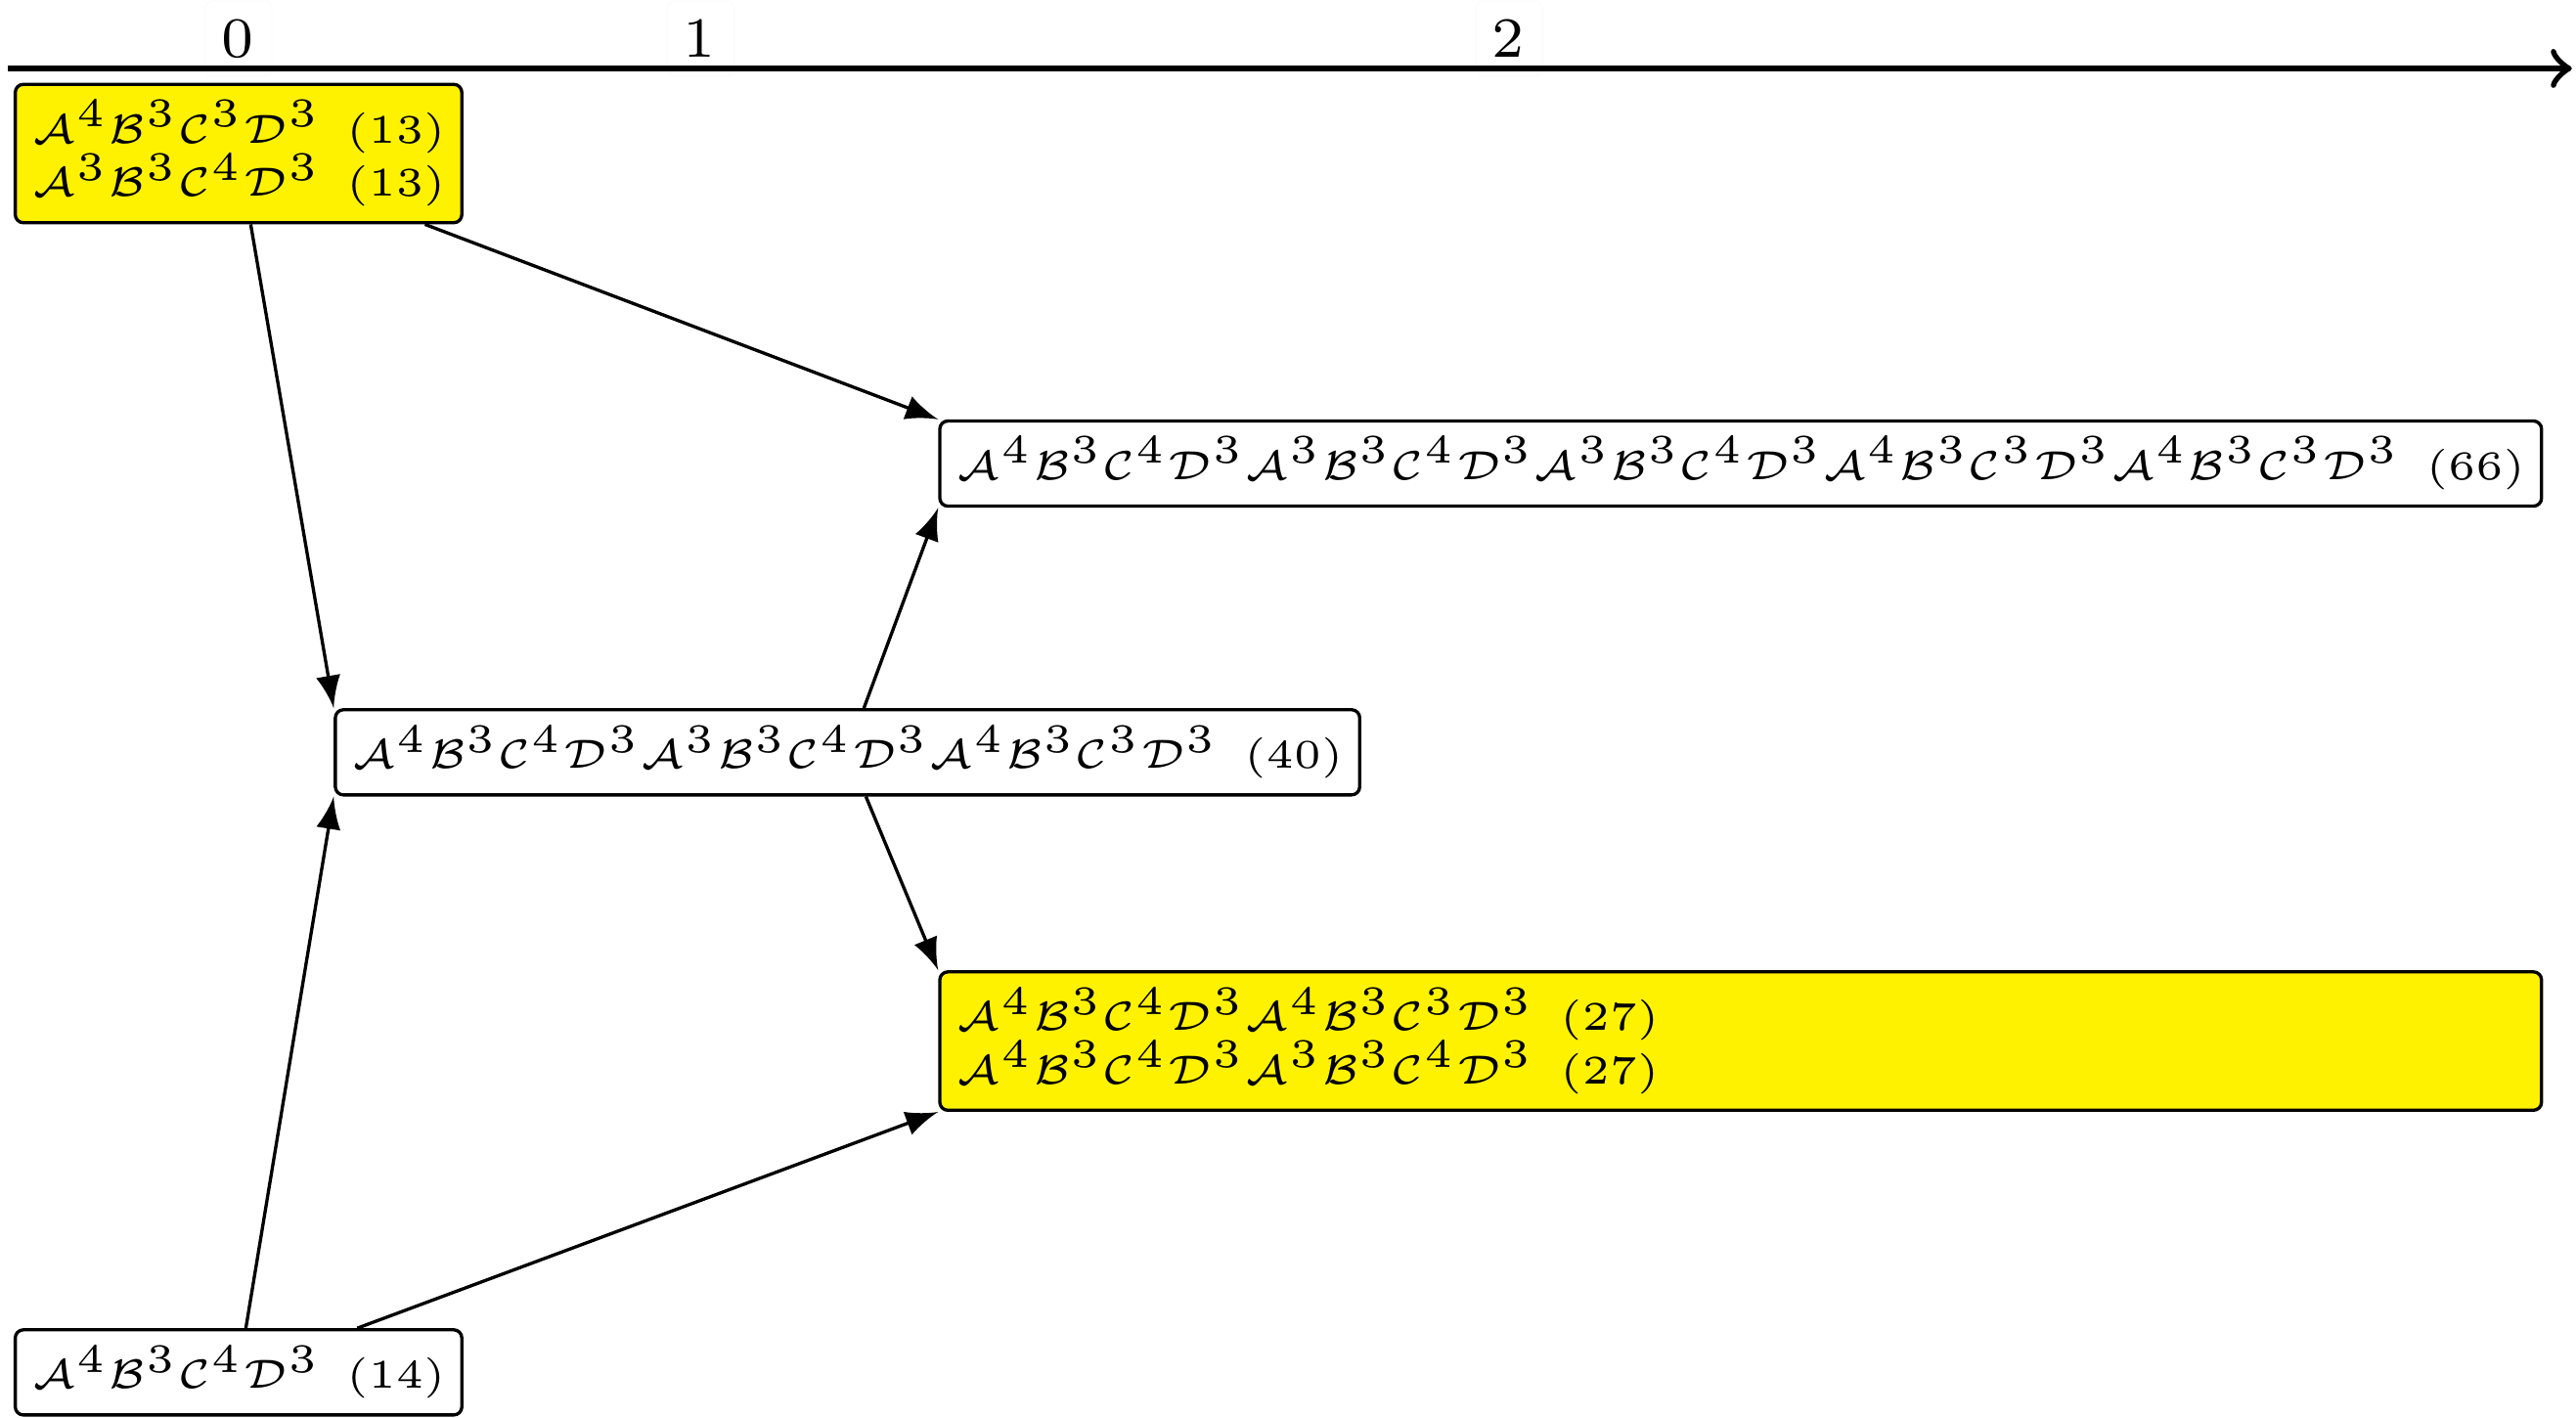
\includegraphics[width=.7 \textwidth]{Figs/Trees/FullArchetypal/adding.png}
		\end{figure}
	}
\end{frame}

\begin{frame}{Halved Model}
	\vspace{-1em}
	\begin{columns}
		\begin{column}{.4 \textwidth}
			\begin{figure}
				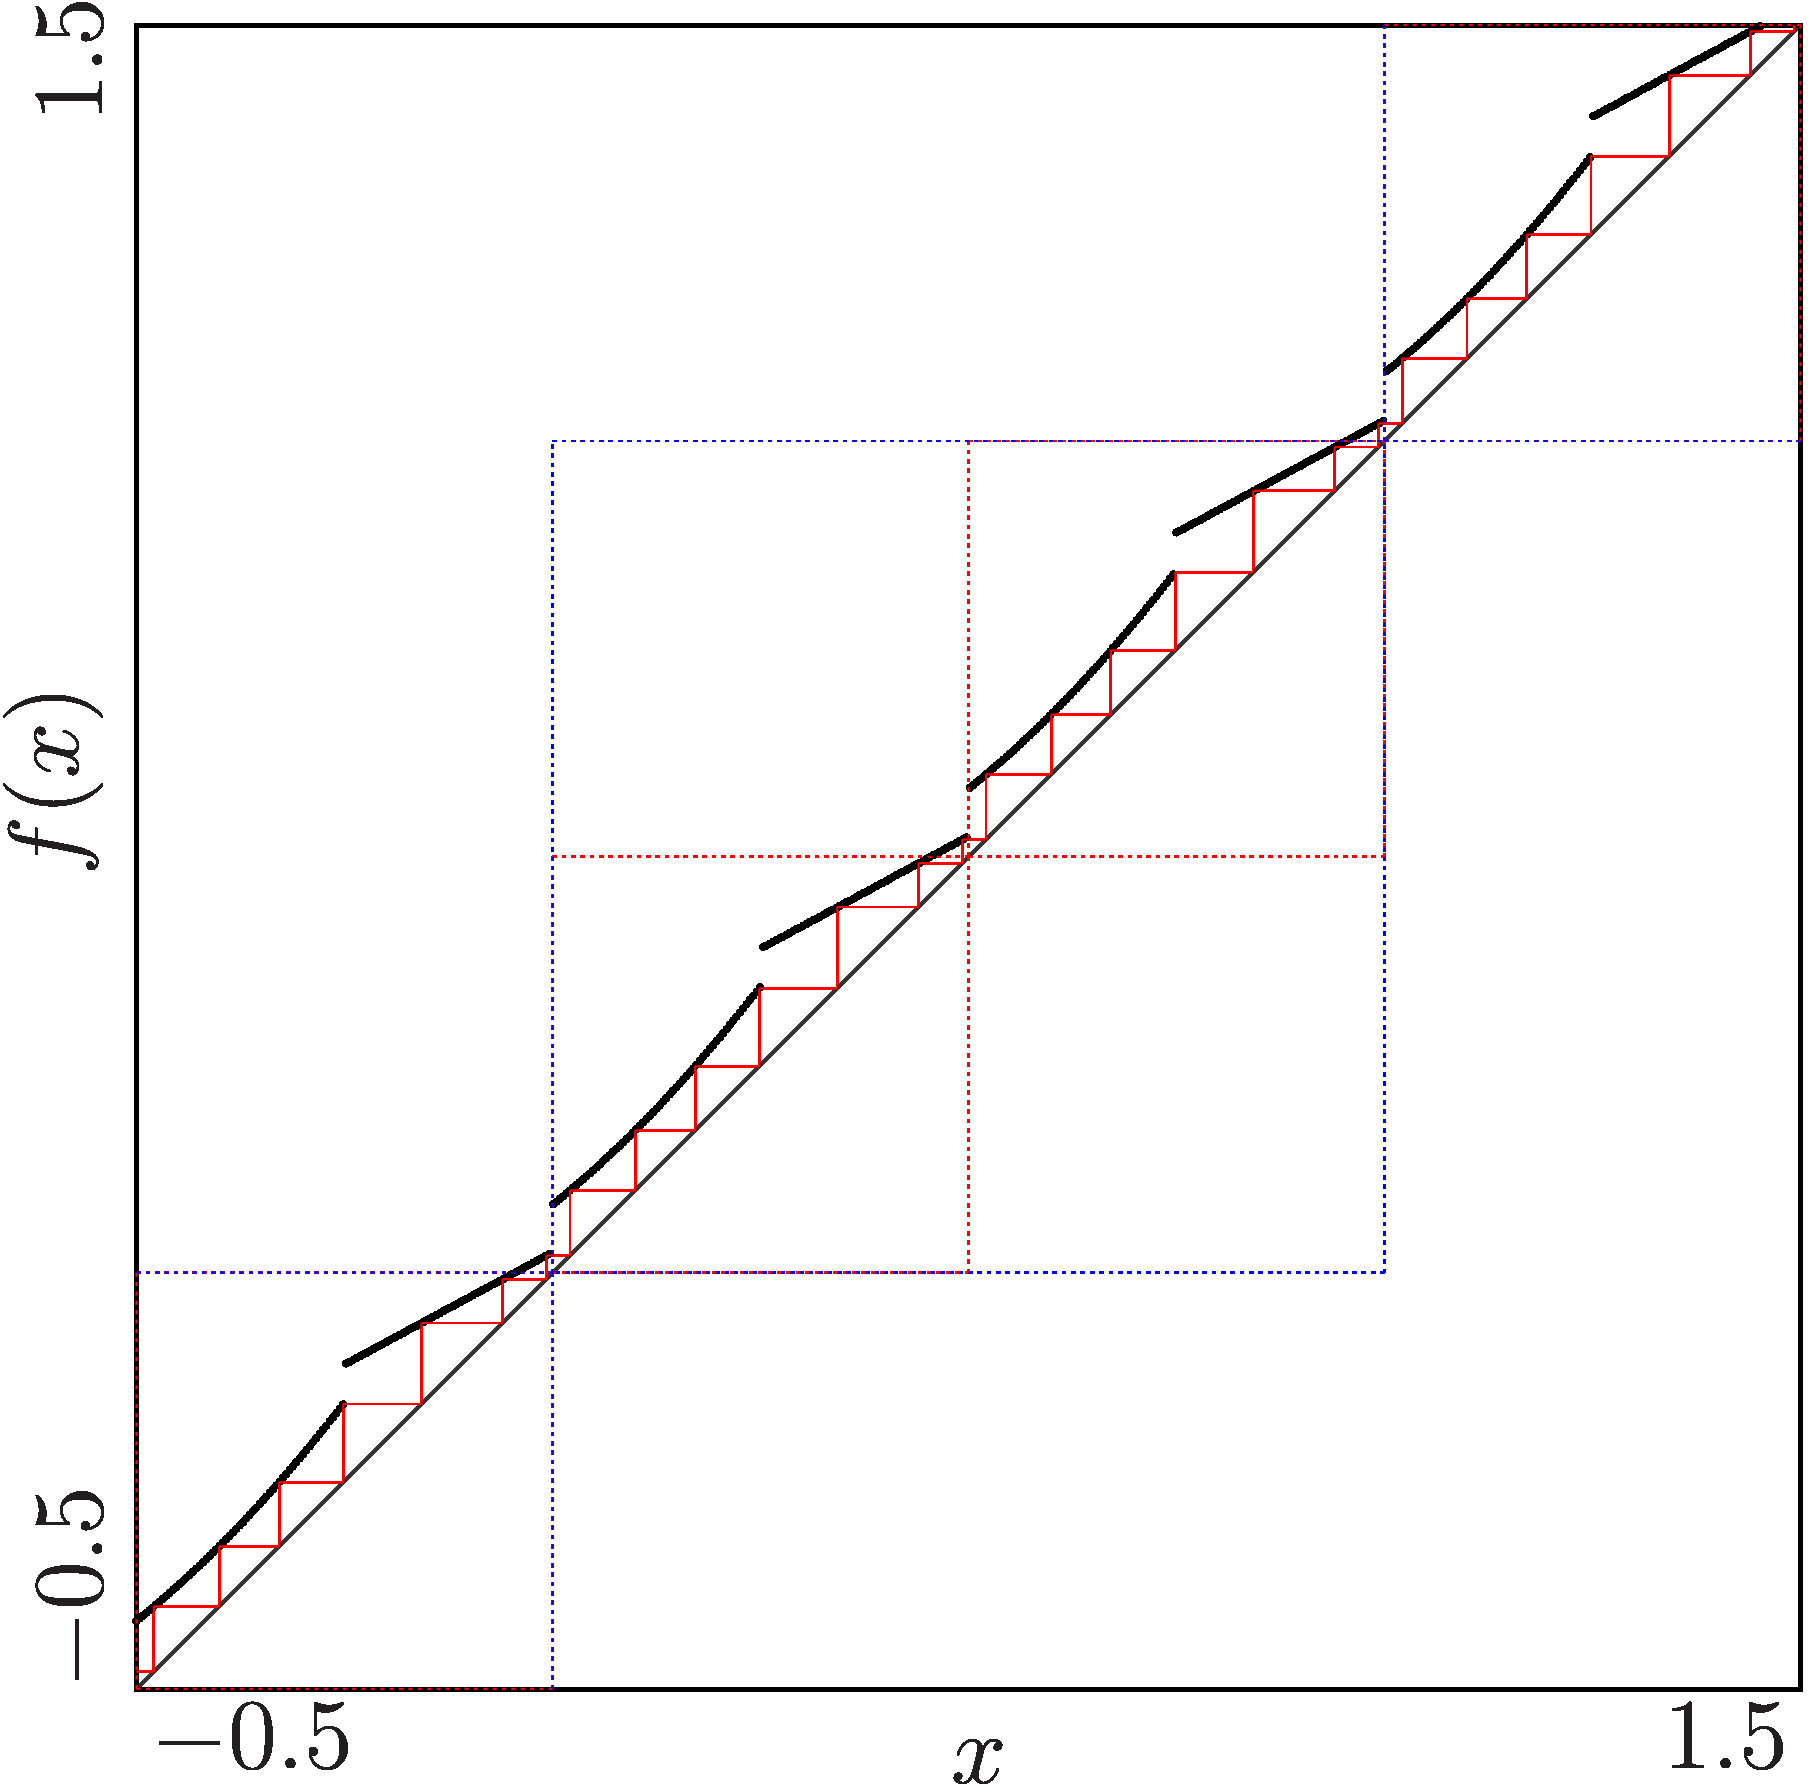
\includegraphics[width=\textwidth]{Figs/archetypal_model_lifted.png}
			\end{figure}
		\end{column}
		\begin{column}{.5 \textwidth}
			\begin{itemize}
				\item Lift the model from $[0, 1)$ to $\mathbb{R}$
				      %\item The lifted model repeats every $1$ step
				      %\item But it even repeats every $\frac{1}{2}$ step because of the built-in symmetry
				\item Drop the model to $[0, \frac{1}{2})$
				\item[$\Rightarrow$] Halved Model
			\end{itemize}
			\begin{align*}
				x    & \mapsto g(x) \mod \frac{1}{2}                                              \\
				g(x) & = \begin{cases}
					         g_L(x) = a_L \cdot x^2 + b_L \cdot x + c_L & \text{ if } x < \frac{1}{4} \\
					         g_R(x) = b_R \cdot x + c_R                 & \text{ else}
				         \end{cases}
			\end{align*}
		\end{column}
	\end{columns}
\end{frame}

\begin{frame}{Period Adding}
	\only<1>{
		\vspace{-1em}
		\begin{figure}
			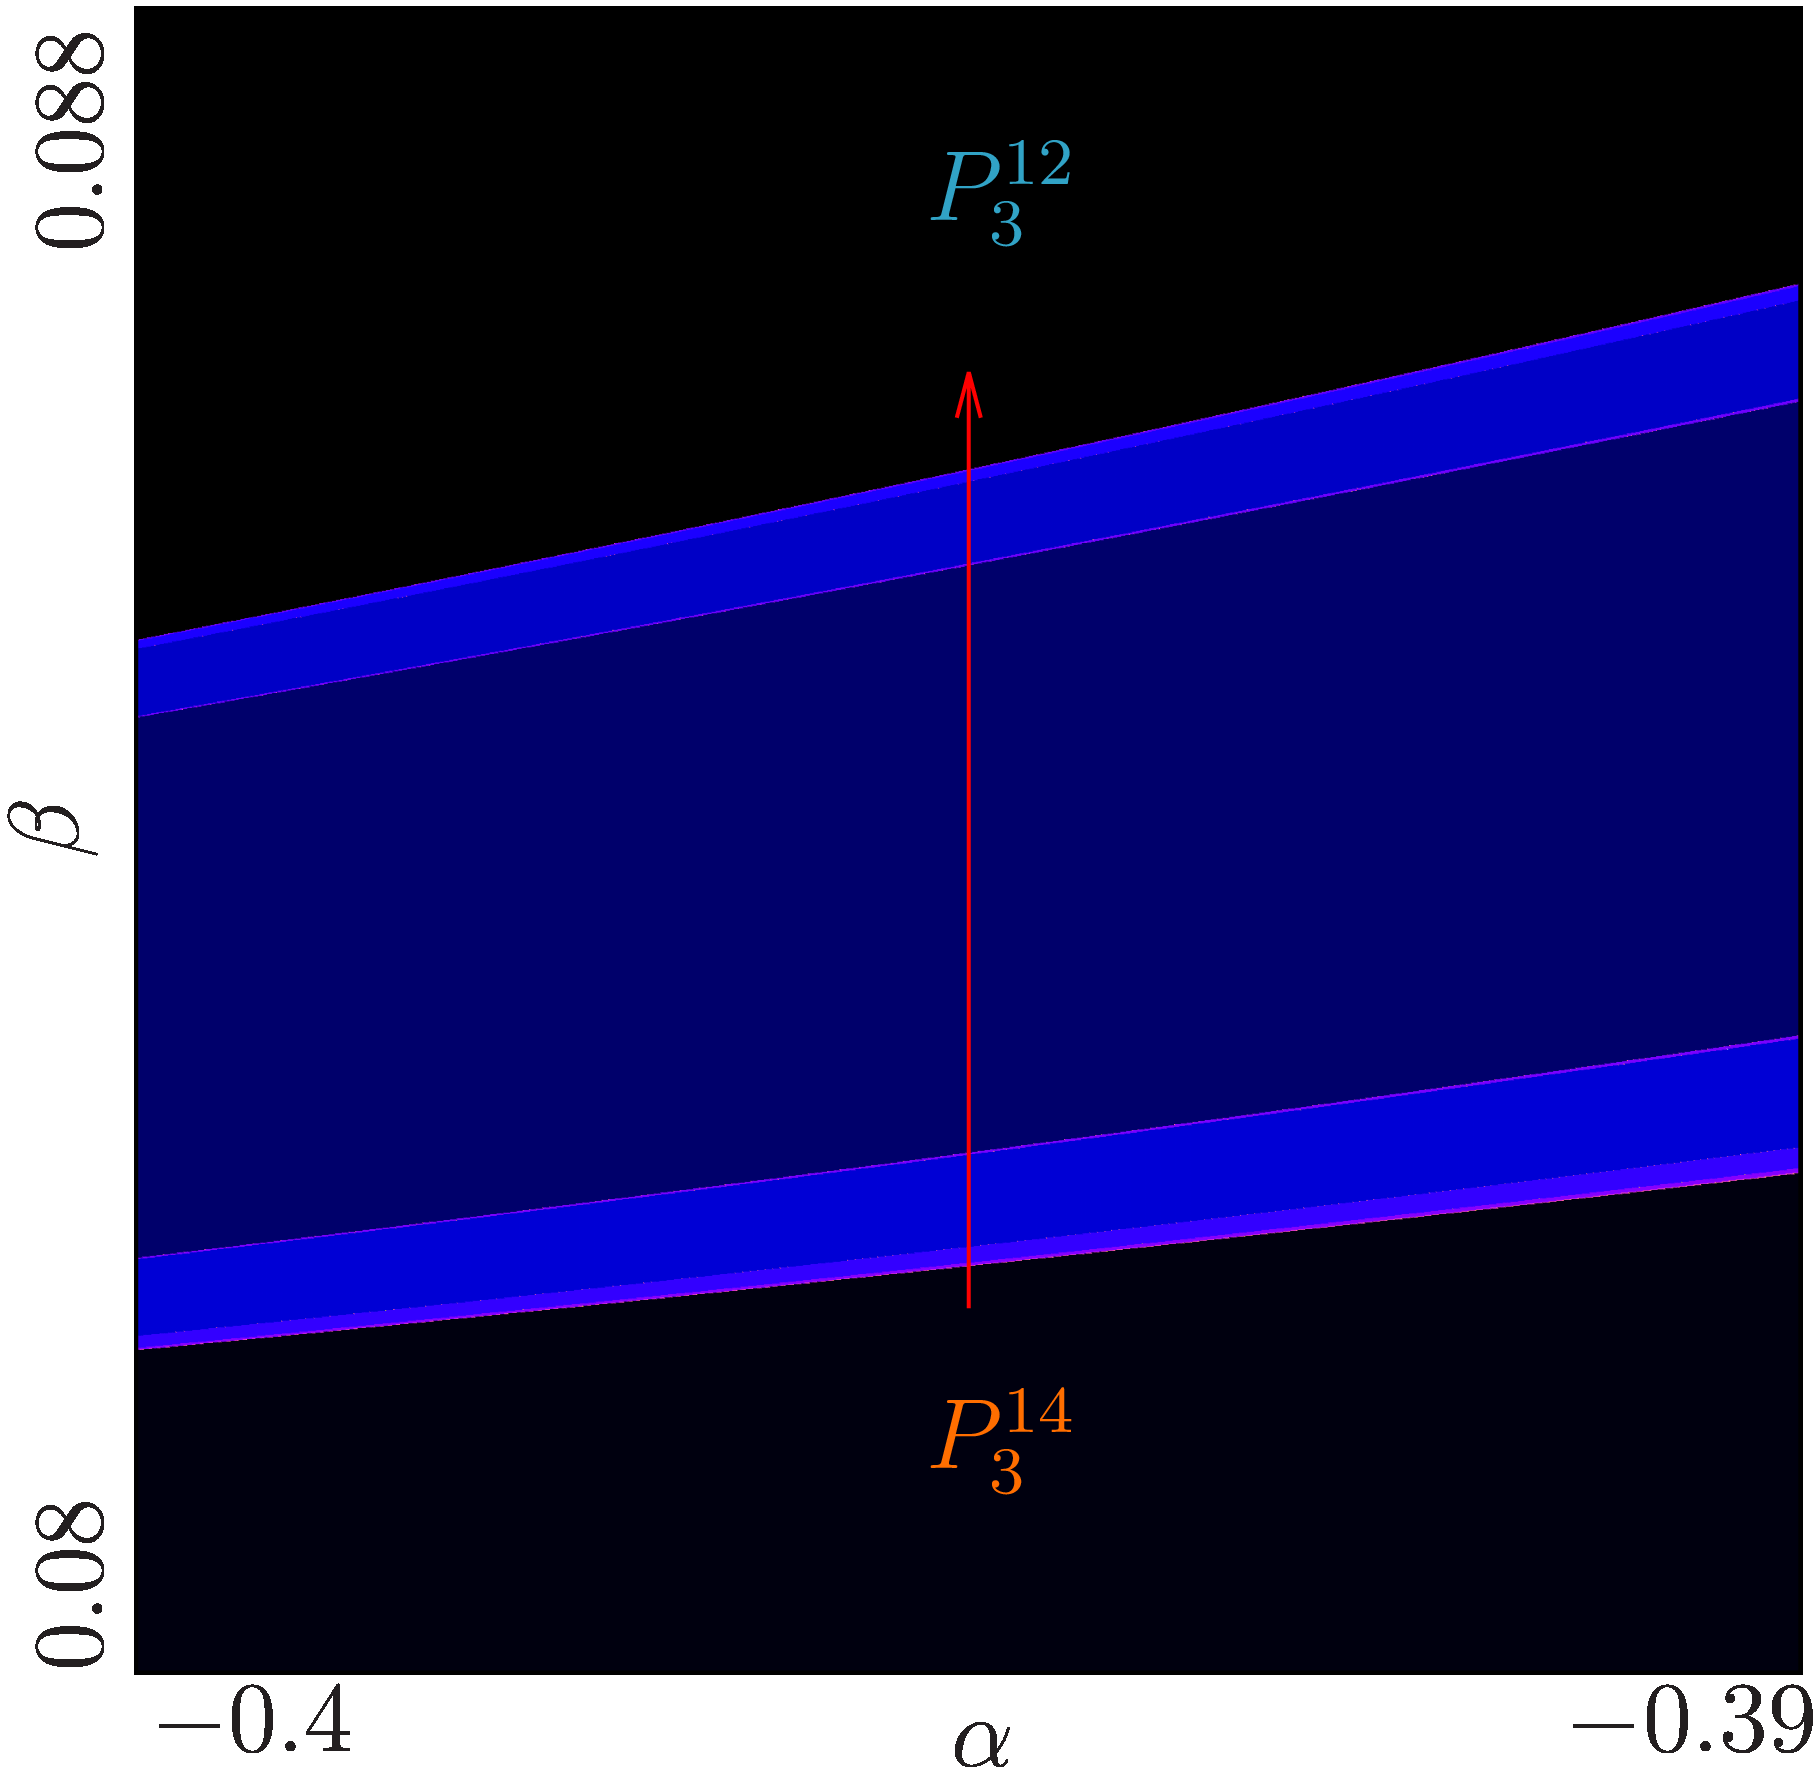
\includegraphics[width=.4 \textwidth]{Figs/archetypal_model_halved_add_hor_2D.png}
			\quad
			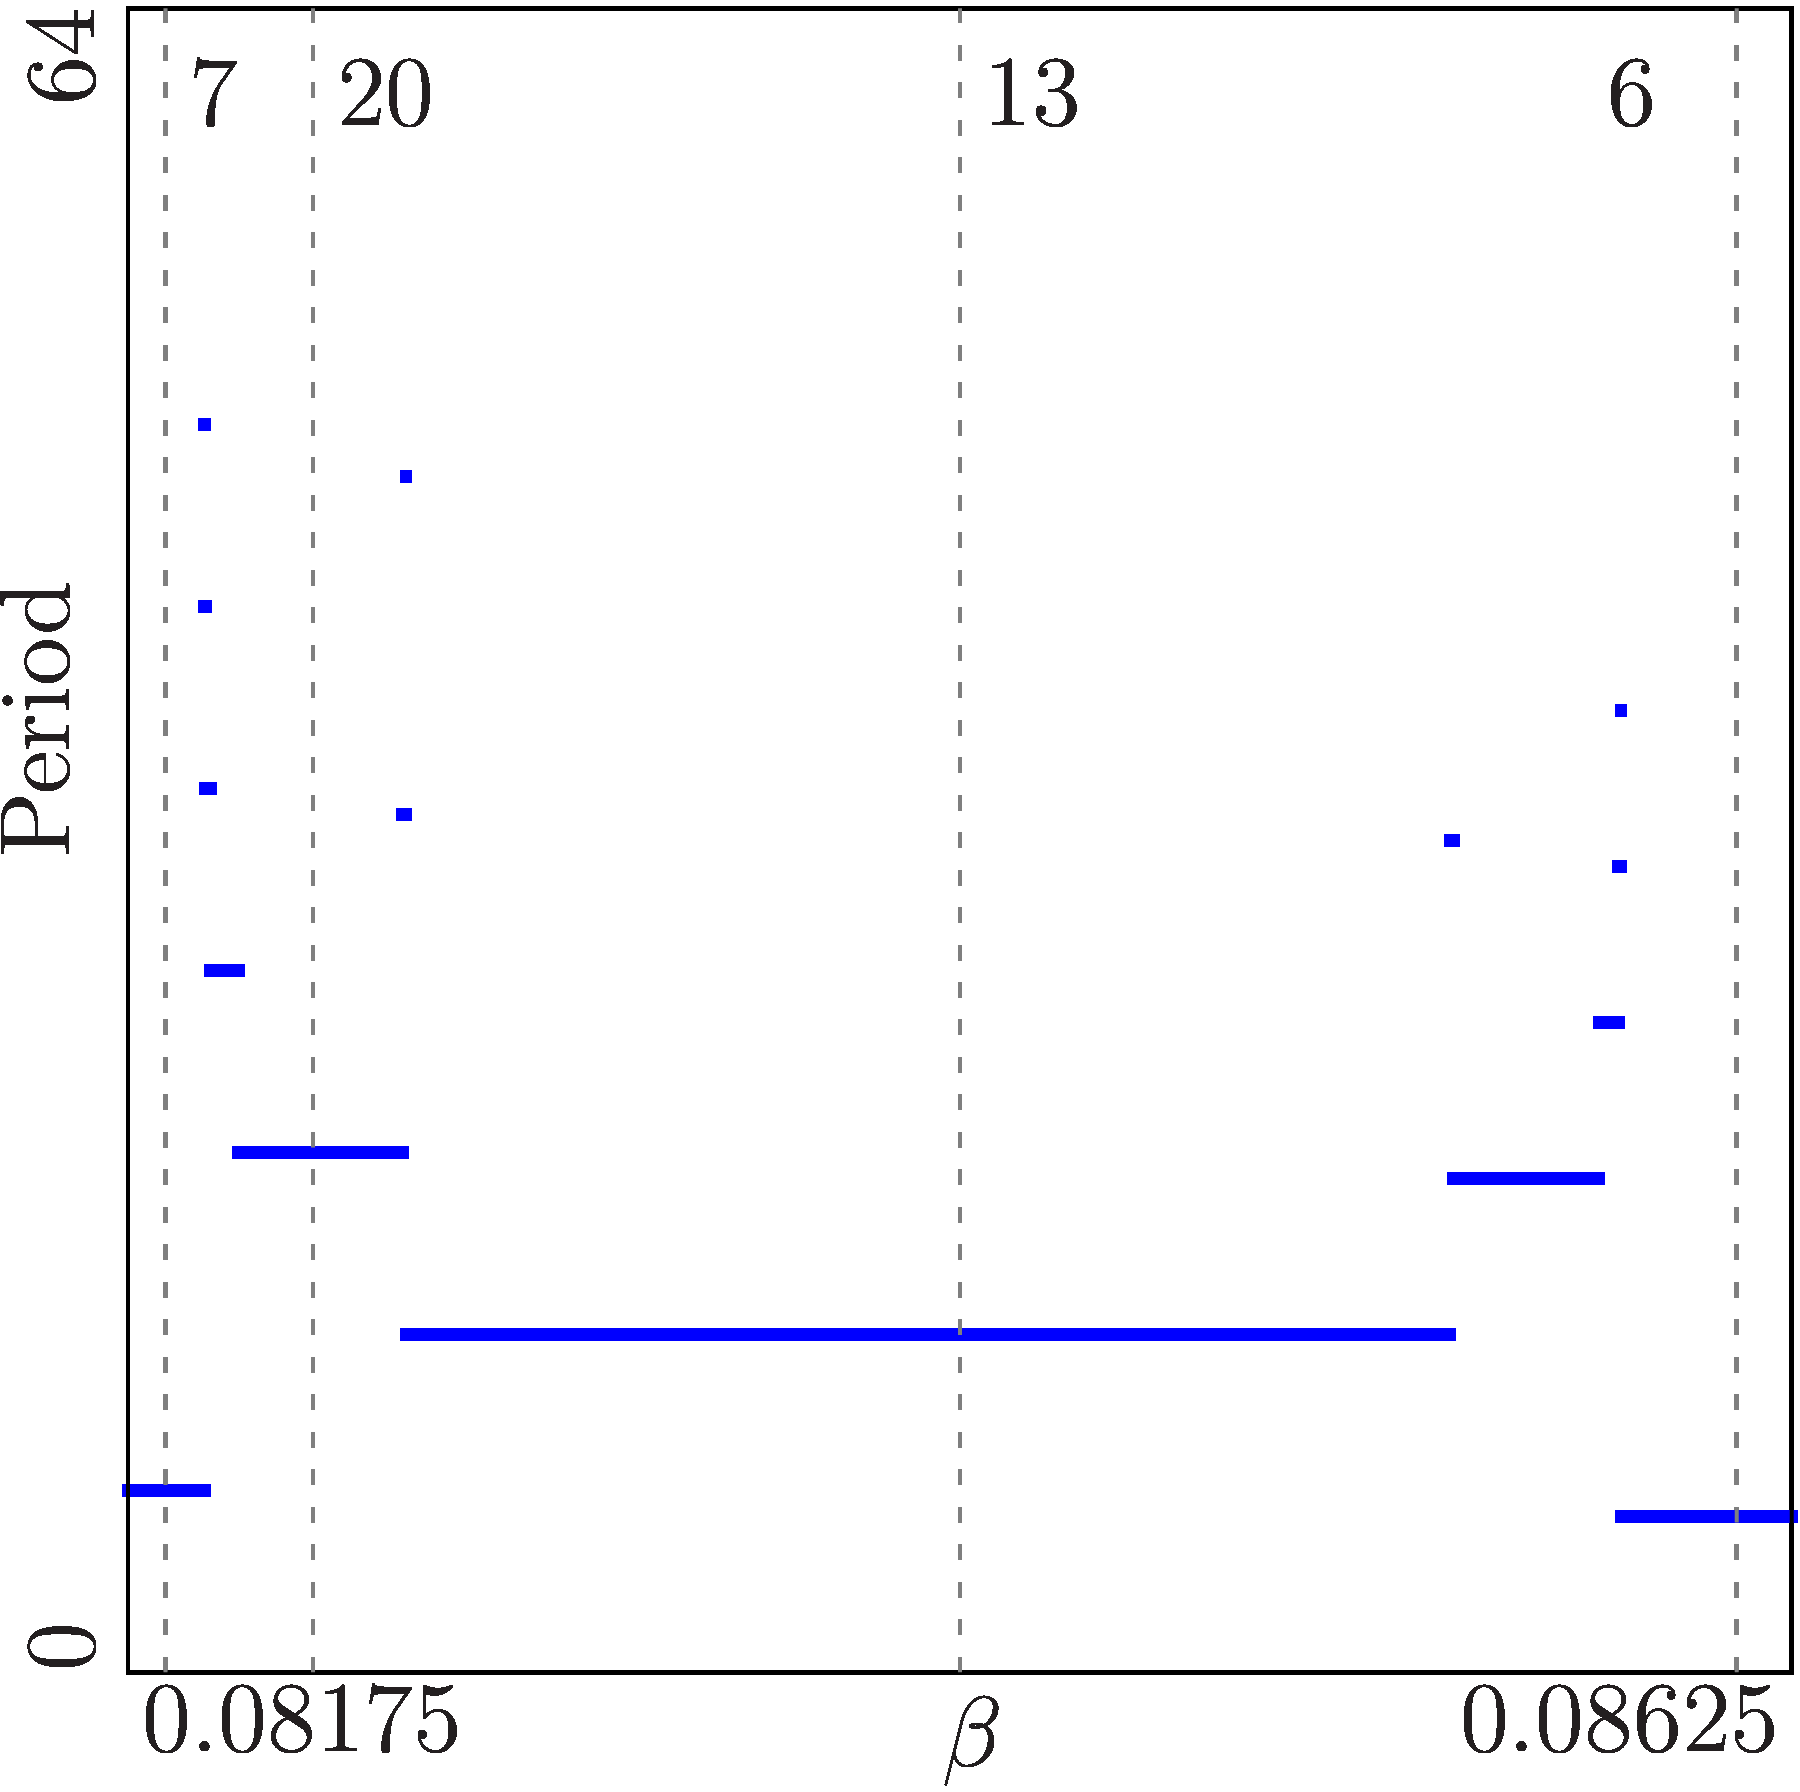
\includegraphics[width=.4 \textwidth]{Figs/archetypal_model_halved_add_hor_1D.png}
		\end{figure}
	}
	\only<2>{
		\vspace{-1em}
		\begin{figure}
			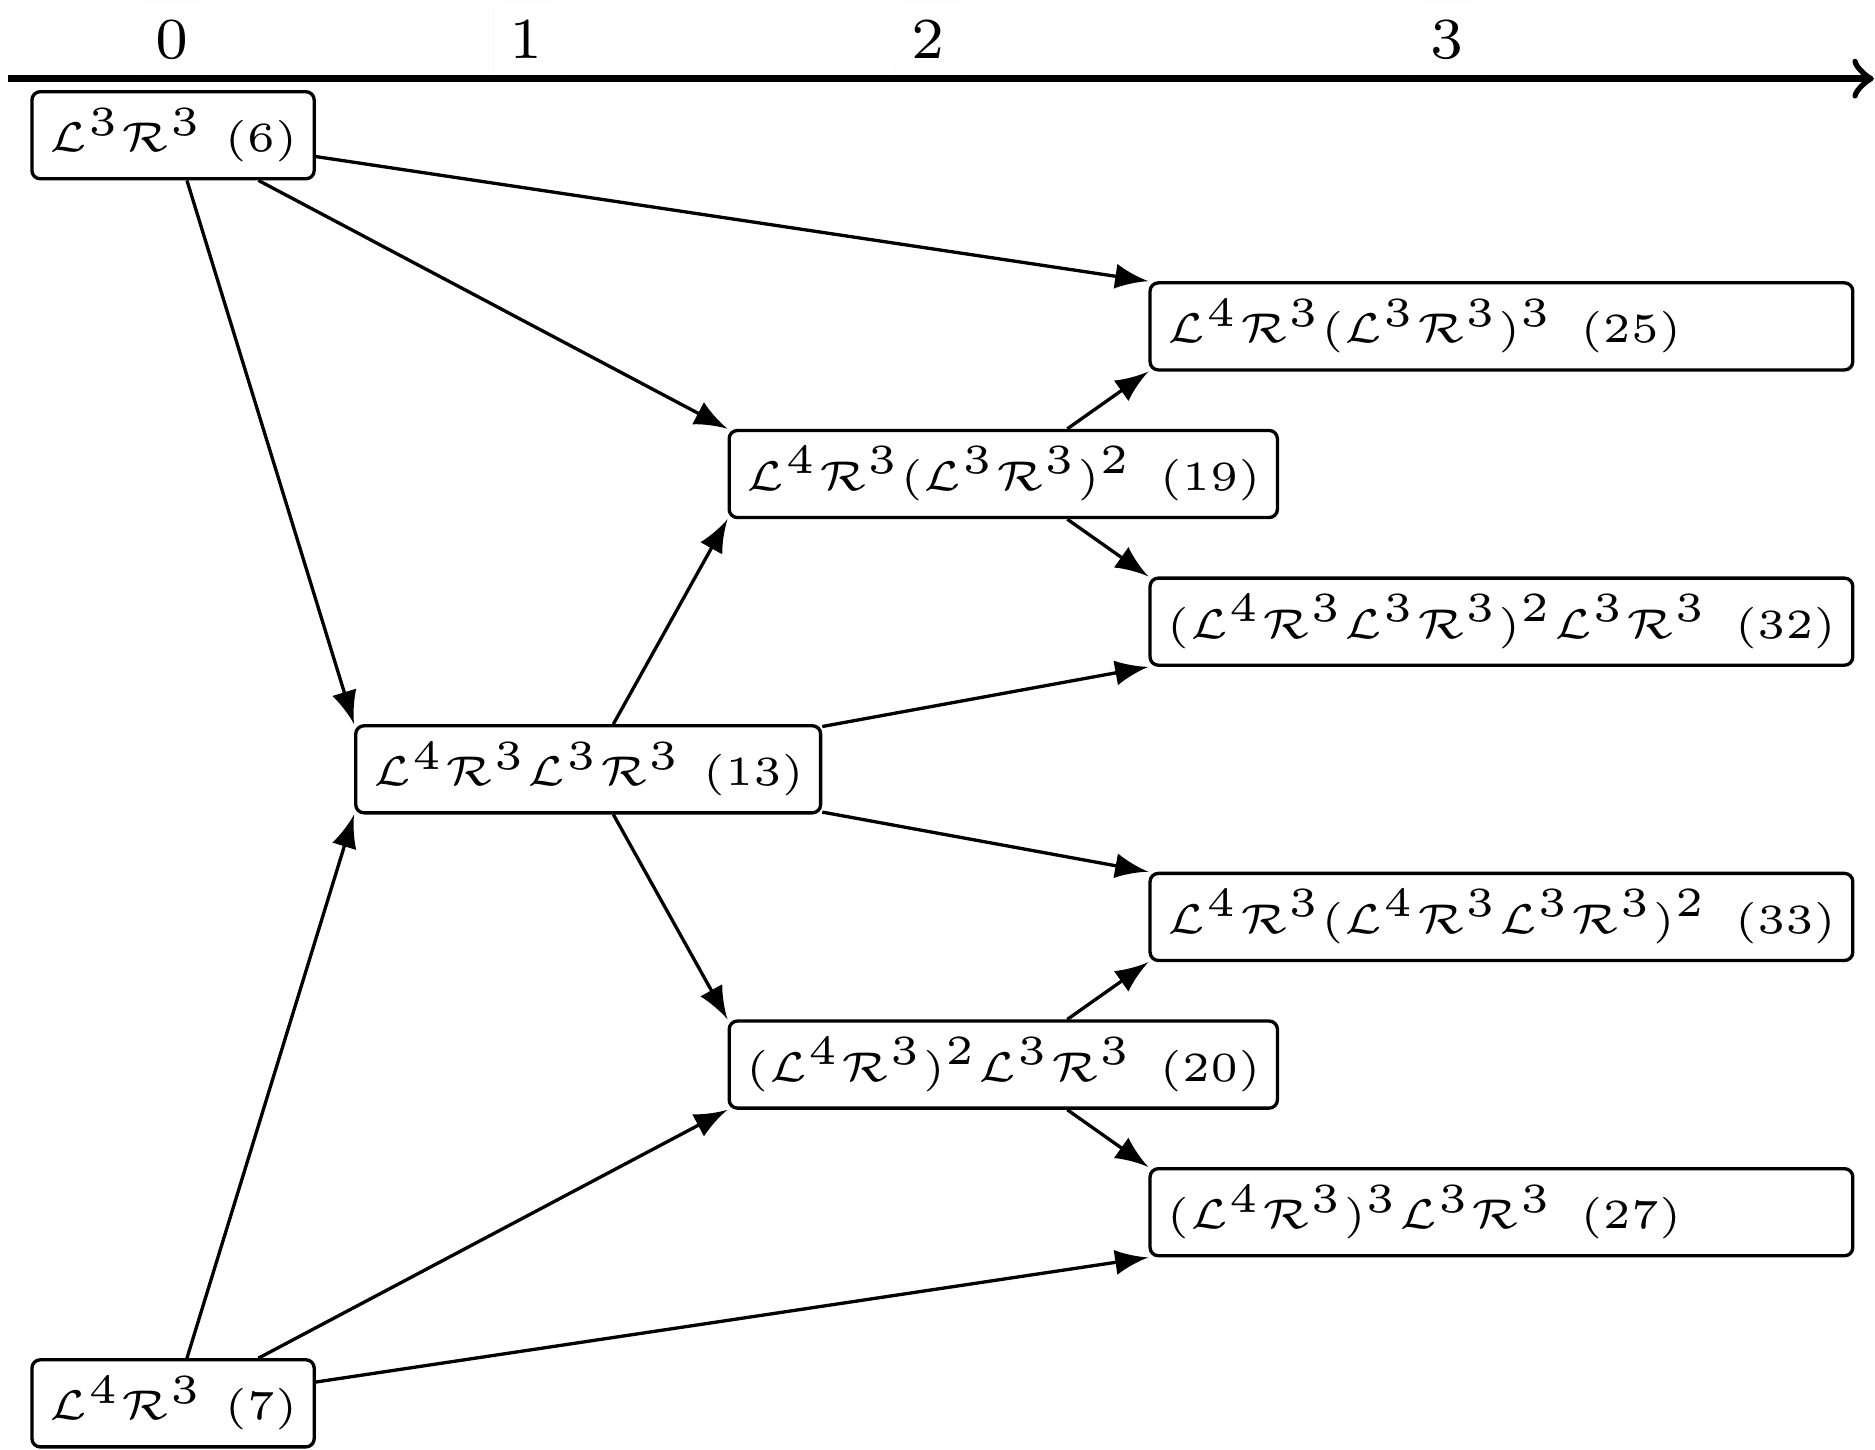
\includegraphics[width=.6 \textwidth]{Figs/Trees/HalvedArchetypal/adding.png}
		\end{figure}
	}
\end{frame}

\begin{frame}{Period Adding Results}
	\vspace{-1em}
	\begin{center}
		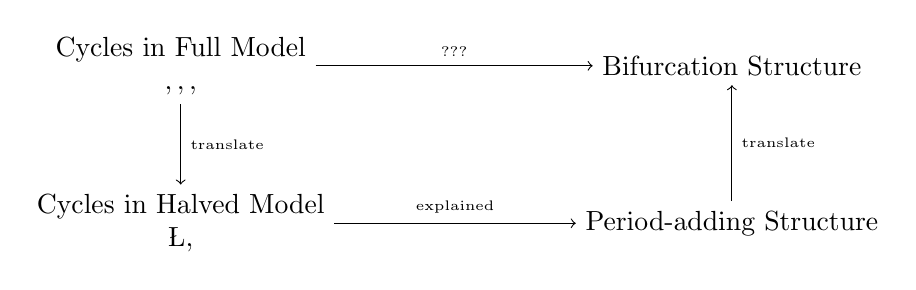
\begin{tikzpicture}[every text node part/.style={align=center}]
			\node (FC) at (0, 2) {Cycles in Full Model \\ $\A, \B, \C, \D$};
			\node (FB) at (7, 2) {Bifurcation Structure};

			\node (HC) at (0, 0) {Cycles in Halved Model \\ $\L, \R$};
			\node (HA) at (7, 0) {Period-adding Structure};

			\draw[->] (FC) -- (HC) node[midway,right] {\tiny translate};
			\draw[->] (HC) -- (HA) node[midway,above] {\tiny explained};
			\draw[->] (HA) -- (FB) node[midway,right] {\tiny translate};
			\draw[->] (FC) -- (FB) node[midway,above] {\tiny ???};
		\end{tikzpicture}
	\end{center}

	\begin{itemize}
		\item Algorithms for translating cycles between both models
		\item Formal description of novel bifurcation structure
		      \begin{itemize}
			      \item When do cycles coexist?
			      \item Symbolic Sequences
			      \item Periods
			      \item Rotation Numbers (here tuples)
		      \end{itemize}
	\end{itemize}
\end{frame}

\begin{frame}{Translation of Symbolic Sequences [Type A]}
	\centering
	\begin{tikzpicture}[thick,scale=1, every node/.style={font=\huge}]
		\path[draw=none] (0,0) -- (12,2);
		%
		\coordinate (a) at (6, 0);
		\coordinate (b) at (6, -2);
		%
		% A1B2C1D2 -> L1R2
		%
		\only<1-4>{
			\node (cycleA) at (a) {$\A^{1}\B^{2}\C^{1}\D^{2}$};
		}
		\only<2>{
			\draw [decorate,decoration={brace,mirror}] (4.3, -0.8) -- (7.7, -0.8);
			\node at (6, -1.5) {4-Silbe};
		}
		\only<3>{
			\node (cycleB) at (b) {$\L^{1}\R^{2}\L^{1}\R^{2}$};
		}
		\only<4>{
			\node (cycleB) at (b) {$\L^{1}\R^{2}$};
		}
		\only<3-4>{
			\draw[->] (cycleA) -- (cycleB);
		}
		%
		% L1R2
		%
		\only<5-8>{
			\node (cycleA) at (a) {$\L^{1}\R^{2}$};
		}
		\only<6>{
			\draw [decorate,decoration={brace,mirror}] (5.0, -0.8) -- (7.0, -0.8);
			\node at (6, -1.5) {2-Silbe};
		}
		\only<7-8>{
			\node (cycleB) at (b) {$\A^{1}\B^{2}$};
		}
		\only<8>{
			\node at (8, -2) {???};
		}
		\only<9>{
			\node (cycleA) at (a) {$\L^{1}\R^{2}\L^{1}\R^{2}$};
			\node (cycleB) at (b) {$\A^{1}\B^{2}\C^{3}\D^{4}$};
		}
		\only<7-9>{
			\draw[->] (cycleA) -- (cycleB);
		}
		%
	\end{tikzpicture}
\end{frame}

%\begin{frame}{Translation of Symbolic Sequences [Full to Halved]}
%	\vspace{3em}
%	\centering
%	\begin{tikzpicture}[thick,scale=1, every node/.style={font=\huge}]
%		\coordinate (a) at (0, 0);
%		\coordinate (b) at (0, -2);
%		\only<1-2>{
%			\node (sigma) at (a) {$\A^{1}\B^{2}\C^{1}\D^{2}$};
%		}
%		\only<1>{
%			\node (phi) at (b) {$\L^{1}\R^{2}\L^{1}\R^{2}$};
%		}
%		\only<2>{
%			\node (phi) at (b) {$\L^{1}\R^{2}$};
%		}
%		\only<3>{
%			\node (sigma) at (a) {$\A^{1}\B^{2}\C^{3}\D^{4}$};
%			\node (phi) at (b) {$\L^{1}\R^{2}\L^{3}\R^{4}$};
%		}
%		\only<4-5>{
%			\node (sigma) at (a) {$\A^{1}\B^{2}\C^{3}\D^{4}\A^{5}\B^{6}\C^{1}\D^{2}\A^{3}\B^{4}\C^{5}\D^{6}$}};
%		\only<4>{
%			\node (phi) at (b) {$\L^{1}\R^{2}\L^{3}\R^{4}\L^{5}\R^{6}\L^{1}\R^{2}\L^{3}\R^{4}\L^{5}\R^{6}$};
%		}
%		\only<5>{
%			\node (phi) at (b) {$\L^{1}\R^{2}\L^{3}\R^{4}\L^{5}\R^{6}$};
%		}
%		\draw[->] (sigma) -- (phi);
%	\end{tikzpicture}
%\end{frame}

%\begin{frame}{Translation of Symbolic Sequences [Halved to Full]}
%	\vspace{3em}
%	\centering
%	\begin{tikzpicture}[thick,scale=1, every node/.style={font=\huge}]
%		\coordinate (a) at (0, 0);
%		\coordinate (b) at (0, -2);
%		\only<1-2>{
%			\node (phi) at (a) {$\L^{1}\R^{2}$};
%		}
%		\only<2>{
%			\node (sigma) at (b) {$\A^{1}\B^{2}$};
%		}
%		\only<4>{
%			\node (phi) at (a) {$\L^{1}\R^{2}\L^{1}\R^{2}$};
%		}
%		\only<4>{
%			\node (sigma) at (b) {$\A^{1}\B^{2}\C^{1}\D^{2}$};
%		}
%		%
%		\only<5>{
%			\node (phi) at (a) {$\L^{1}\R^{2}\L^{3}\R^{4}$};
%			\node (sigma) at (b) {$\A^{1}\B^{2}\C^{3}\D^{4}$};
%		}
%		\only<6>{
%			\node (phi) at (a) {$\L^{1}\R^{2}\L^{3}\R^{4}\L^{5}\R^{6}\L^{1}\R^{2}\L^{3}\R^{4}\L^{5}\R^{6}$};
%		}
%		\only<7>{
%			\node (phi) at (a) {$\L^{1}\R^{2}\L^{3}\R^{4}\L^{5}\R^{6}$};
%		}
%		\only<6-7>{
%			\node (sigma) at (b) {$\A^{1}\B^{2}\C^{3}\D^{4}\A^{5}\B^{6}\C^{1}\D^{2}\A^{3}\B^{4}\C^{5}\D^{6}$}};
%		\only<2-3>{
%			\draw[->] (phi) -- (sigma);
%		}
%	\end{tikzpicture}
%\end{frame}


\begin{frame}{Coexistence of Cycles}
	\begin{itemize}
		\item Oddly enough, coexistence more natural
		\item Odd number of rotations (in halved model) $\Rightarrow$ No coexistence (in full model)
		      \vspace{1em}
		\item Child of two nodes with coexistence has no coexistence
		\item Child of two nodes with no coexistence has no coexistence
		\item Child of a node with and a node with no coexistence has coexistence
	\end{itemize}

\end{frame}

%%% Local Variables:
%%% mode: latex
%%% TeX-master: "../Vortrag_Frauenhofer_Weik"
%%% End:
